\part{Quantile and Distribution Regression}
 
 As \cite{Heckman1997} point out, often interest lies in 
 
\section{Preliminaries: Quantiles and Their Properties}
 \label{quantile:section:quantile_properties}


\subsection{Definition and Basic Properties}
 
 We begin by formally defining the quantile function and establishing some of its basic properties.  
 \begin{dfn}
 	\label{quantile:definition:quantile_function}
 	Let $F$ be a cumulative distribution function on the real line. Then its quantile function $Q:(0, 1)\to \R$ is the generalized inverse
 	\begin{equation}
 		Q(\tau) = \inf\curl*{ x: F(x)\geq \tau }.
 	\end{equation}
 \end{dfn}
 The quantile function is typically labeled $F^{-1}(\tau)$ or $Q(\tau)$. 
 %
% In this section, we will mostly use the $F^{-1}(\cdot)$ to emphasize the connection with $F$. 
 %
% However, we will switch to the less burdensome $Q(\cdot)$ notation when working with conditional quantiles. 
 
 Fig. \ref{quantile:figure:quantile_drawing}  provides a graphical representation of the quantile function. The left plot depicts an example distribution function $F$. The right plot depicts the quantile function $Q$. This plot is obtained by simply reflecting the CDF plot along the 45 degree line. 
  
 \begin{figure}[ht!]
 	
 	\centering 
 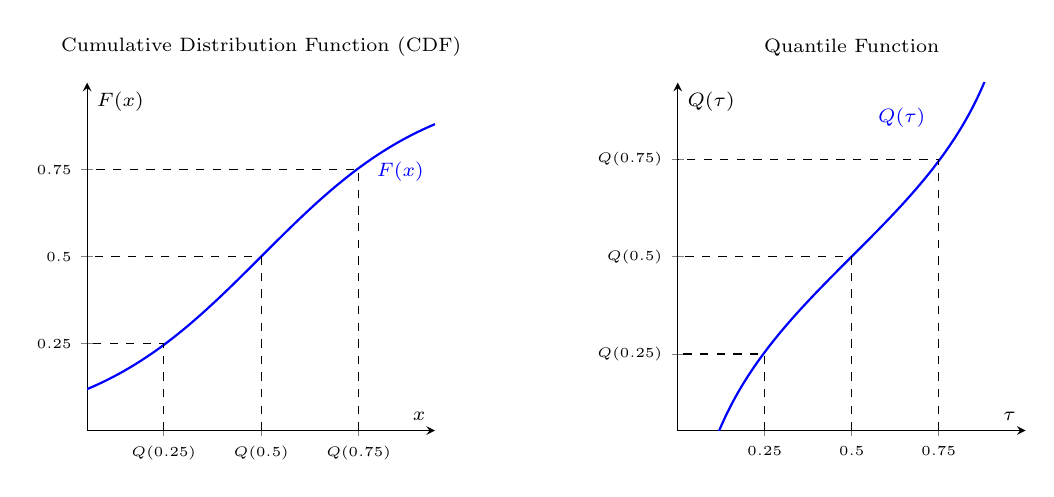
\begin{tikzpicture}
 	
 	    \def\xA{2.2}  % Approximate x for Q(0.25)
 	\def\xB{5}  % Approximate x for Q(0.5) (median)
 	\def\xC{7.8}  % Approximate x for Q(0.75)
 	
 	% First frame: CDF plot (left side)
 	\begin{axis}[
 		width=6cm, height=6cm,
 		xmin=0, xmax=10,
 		ymin=0, ymax=1,
 		axis lines=middle,
 		xlabel={$x$},
 		ylabel={$F(x)$},
 		xtick={\xA,5,\xC},
 		ytick={0.25,0.5,0.75},
 		xticklabels={$Q(0.25)$, $Q(0.5)$, $Q(0.75)$},
 		yticklabels={$0.25$, $0.5$, $0.75$},
 		domain=0:10,
 		samples=100,
 		smooth,
 		title={\scriptsize Cumulative Distribution Function (CDF)},
 		label style={font=\scriptsize},
 		tick label style={font=\tiny}
 		]
 		
 		% Plot the CDF-like function (using a logistic function as an approximation)
 		\addplot[blue, thick] {1 / (1 + exp(-0.4 * (x - 5)))};
 		
 		% Draw dashed lines for each quantile level
 		\draw[dashed] (axis cs:\xA, 0) -- (axis cs:\xA, 0.25) -- (axis cs:0, 0.25) node[left, font=\scriptsize] {$0.25$};
 		\draw[dashed] (axis cs:\xB, 0) -- (axis cs:5, 0.5) -- (axis cs:0, 0.5) node[left, font=\scriptsize] {$0.5$};
 		\draw[dashed] (axis cs:\xC, 0) -- (axis cs:\xC, 0.75) -- (axis cs:0, 0.75) node[left, font=\scriptsize] {$0.75$};
 		
 		% Label the quantile points on the x-axis
 		\node[below, font=\scriptsize] at (axis cs:2, 0) {$Q(0.25)$};
 		\node[below, font=\scriptsize] at (axis cs:5, 0) {$Q(0.5)$};
 		\node[below, font=\scriptsize] at (axis cs:8, 0) {$Q(0.75)$};
 		
 		% Add a label for the CDF curve
 		\node at (axis cs:9,0.8) [below, font=\scriptsize, blue] {$F(x)$};
 		
 	\end{axis}
 	
 	% Second frame: Quantile function plot (right side, shifted)
 	\begin{axis}[
 		at={(7.5cm,0)}, % Horizontal shift to place next to the CDF plot
 		width=6cm, height=6cm,
 		xmin=0, xmax=1,
 		ymin=0, ymax=10,
 		axis lines=middle,
 		xlabel={$\tau$},
 		ylabel={$Q(\tau)$},
 		xtick={0.25,0.5,0.75},
 		ytick={\xA,5,\xC},
 		xticklabels={$0.25$, $0.5$, $0.75$},
 		yticklabels={$Q(0.25)$, $Q(0.5)$, $Q(0.75)$},
 		domain=0:1,
 		samples=100,
 		smooth,
 		title={\scriptsize Quantile Function},
 		label style={font=\scriptsize},
 		tick label style={font=\tiny}
 		]
 		
 		% Plot the inverse CDF function (quantile function)
 		\addplot[blue, thick] {5 + ln(x / (1 - x)) / 0.4};
 		
 		% Draw dashed lines for each probability level
 		\draw[dashed] (axis cs:0.25, 0) -- (axis cs:0.25, \xA) -- (axis cs:0, \xA) node[left, font=\scriptsize] {$Q(0.25)$};
 		\draw[dashed] (axis cs:0.5, 0) -- (axis cs:0.5, 5) -- (axis cs:0, 5) node[left, font=\scriptsize] {$Q(0.5)$};
 		\draw[dashed] (axis cs:0.75, 0) -- (axis cs:0.75, \xC) -- (axis cs:0, \xC) node[left, font=\scriptsize] {$Q(0.75)$};
 		
 		% Label the probability points on the x-axis
 		\node[below, font=\scriptsize] at (axis cs:0.25, 0) {$0.25$};
 		\node[below, font=\scriptsize] at (axis cs:0.5, 0) {$0.5$};
 		\node[below, font=\scriptsize] at (axis cs:0.75, 0) {$0.75$};
 		
 		% Add a label for the quantile function curve
 		\node at (axis cs:0.74,9) [left, font=\scriptsize, blue] {$Q(\tau)$};
 		
 	\end{axis}
 	
 \end{tikzpicture}
 	
 	\caption{Graphic representation of the quantile function. }\label{quantile:figure:quantile_drawing}
 \end{figure}
 
 
 \paragraph{Inequality and composition properties of quantile functions}
 
 
 \begin{cl}[Lemma 21.1 in \cite{VanderVaart1998}]
 	\label{quantile:theorem:basic_properties}
 	Let $F$ be a CDF and $Q$ be its quantile function. Then for all $\tau\in (0, 1)$ and $x\in \R$ it holds that 
 		\begin{enumerate}
 			\item $Q(\cdot)$ is monotonic
 			\item \emph{Galois inequalities}: $Q(\tau)\leq x$ iff $\tau\leq F(x)$
 			\item $Q(\cdot)$ is a left-continuous function with right limits.
% 		\item $A(\tau) = \curl*{s: F(s)\geq \tau }$ is closed

%\item 
\item $Q\circ F(x) \leq x$

 		\item $F\circ Q(\tau)\geq \tau$ % , with equality iff $\tau$ is in range of $F$. Equality can only fail if $F$ is discontinuous at $F^{-1}(\tau)$

%\item $F\circ F^{-1}(\tau) \leq \tau$ 
 	\end{enumerate}
 \end{cl}
 
 \begin{proof}
 	
 	We prove the assertions in the same order as they are stated: 
 \begin{enumerate}
 	\item \emph{Monotonicity}: let $\tau_1<\tau_2$. Since $F(x)$ is non-decreasing, it holds that $\curl{x: F(x)\geq \tau_1} \supseteq \curl{x: F(x)\geq \tau_2}$. Accordingly, the infimum over the first set is no greater than the infimum over the second set, that is, $Q(\tau_1)\leq Q(\tau_2)$.
 		\item \emph{Galois inequalities}: first, 	let $Q(\tau)\leq x$. By definition, $x\in \curl{z: F(z)\geq \tau}$, implying that $F(x)\geq \tau$. 
 		%
 		Second, let $\tau\leq F(x)$. Then $x\in\curl{z: F(z)\geq \tau}$, and hence $x\geq \inf_{F(z)\geq \tau} z\equiv Q(\tau)$.
  
%  	For left-continuity, fix $\tau$ and let $\tau_n\uparrow \tau$. \
\item  \emph{Left-continuity}: since $Q(\cdot)$ is a non-decreasing function, it can only have jump discontinuities. It is then sufficient to prove that at every $\tau_0$ it holds that $\sup_{\tau<\tau_0} Q(\tau) = Q(\tau)$. Label $x=\sup_{\tau<\tau_0} Q(\tau)$ and $y=Q(\tau)$.
 %
 By monotonicity, $x\leq y$. Now note that for any $\varepsilon>0$ by definition it holds that $F(x+\varepsilon)\geq \tau_0$. By the Galois inequalities, it holds that $y\leq x+\varepsilon$. Since this inequality holds for any $\varepsilon>0$, we conclude that $y\leq x$, showing that $y=x$, as desired. 
  
  	 \item By construction, $x \in \curl{z: F(z)\geq F(x)}$, hence 
  	 \begin{equation}
  	 	x \geq \inf_{F(z)\geq F(x)} z \equiv Q(F(x)).
  	 \end{equation}
 
 \item Label $x= Q(\tau)$ and  let  $\curl{x_n}_{n=1}^{\infty}$ be a sequence that monotonically decreases to $x$. Then $F(x_n)\geq \tau$ for all $n$. Since $F$ is right-continuous, we conclude that $F(x)\geq \tau$ as well.
 \end{enumerate}
 \end{proof}

 
 
 \paragraph{Corollary: quantiles uniquely determine the distribution}
 
 An important corollary of the above properties is that quantiles uniquely determine distributions.
 \begin{cl}
 	Quantiles uniquely determine the distribution.
 \end{cl}
 
 \begin{proof}
 	Let $F_1(\cdot)$ and $F_2(\cdot)$ be two CDFs with $Q_1(\cdot) = Q_2(\cdot)$. 
 	%
 	Let $x$ be arbitrary.  Then by (4) in result \ref{quantile:theorem:basic_properties} it holds that 
 	$Q_2(F_2(x)) \leq x$. By equality of quantiles, $Q_2(F_2(x))=Q_1(F_2(x))$. Applying (2) in result \ref{quantile:theorem:basic_properties} with $\tau = F_2(x)$, we conclude that 
 	\begin{equation}
 		 F_2(x) \leq F_1(x).
 	\end{equation}
 By flipping $F_2$ and $F_1$ in the above argument, we conclude that $F_1(x)\leq F_2(x)$. These two inequalities imply that $F_1(x)= F_2(x)$ at all $x$.
 \end{proof}
 

 \paragraph{Corollary: quantile transformation}
 
 
 Another useful corollary is that any random variable can be constructed using the \emph{quantile transform}: composing a standard uniform random variable with an appropriate quantile function.
 %
 This construction allows for convenient sampling of random variables from any distribution with an available quantile function.
 % 
 It also allows for convenient constructions of random variables on the same probability space (Skorokhod construction).
 \begin{cl}
 	\label{quantile:theorem:quantileTransform}  
 	
 Let $U$ be  a Uniform[0, 1] random variable.  Let $F(\cdot)$ be a CDF with quantile function $Q(\cdot)$. Then $Q(U)$ is a random variable distributed according to $F$. 
 \end{cl}
 
 
 
 \begin{proof}
 By (2) in result \ref{quantile:theorem:basic_properties} it holds that 
 $\curl{Q(U)\leq x} = \curl{U\leq F(x) }$, so $P(Q(U)\leq x) = P(U\leq F(x))= F(x)$, as desired. 
 \end{proof}
 
 
  \paragraph{Corollary: expressing the CDF in terms of quantiles}
 
 Result \ref{quantile:theorem:quantileTransform}  implies an explicit representation for the CDF in terms of the quantiles:
 \begin{align}
 	F(x) & = \E\left[ \I\curl{X\leq x} \right] = \E\left[ \curl{Q(U) \leq x } \right] = \int_{(0, 1)} \I\curl{ Q(\tau)\leq x  }d\tau.
 \end{align}
 This expression can also be used to prove that quantiles uniquely determine distributions.
 
 
 \paragraph{Quantile convergence lemma} 
 
 It turns out that weak convergence of quantile functions is equivalent to weak convergence of the corresponding distribution functions.
 
 \begin{cl}[Lemma 21.2 in \cite{VanderVaart1998}]
%  
Let $\curl{F_n}_{n=1}^{\infty}$ be any sequence of cumulative distribution functions. Then  $F_n\Rightarrow F$ iff $Q_n\Rightarrow Q$. 
 \end{cl}
 A particular application of this results is convergence of critical values. Fix $\alpha \in (0, 1)$ such that $F$ is continuous and strictly increasing at $F^{-1}(1-\alpha)$. Then the above result shows that
 	\begin{equation}
 			Q_n(1-\alpha) \to Q(1-\alpha).
 	\end{equation} 
 	This type of convergence results is particularly useful for describing consistency of bootstrapped critical values.
 
 
 \begin{proof}
  Suppose that $Q_n\Rightarrow Q$. 
  %
  Let $U$ be a Uniform[0, 1] random variable. 
  %
  $Q(\cdot)$ has at most a countable number of discontinuity points.
  %
  Accordingly, $Q_n(U)\to Q(U)$ holds for almost all realizations of $U$ (that is, except those that happen to be equal to the discontinuity points of $Q$).
  % 
  Almost sure convergence implies weak convergence.
  %
  However, the distribution function of $Q_n(U)$ is exactly $F_n$, likewise with $Q(U)$.
  %
  We conclude that $F_n\Rightarrow F$. 
  
  
  \vspace{3mm}
  
  Now suppose that $F_n\Rightarrow F$. 
  %
   Let $V$ be a random normal variable (or any other variable whose CDF is strictly increasing on all of $\R$).
   %
   $F$ has most a countable number of discontinuity points.
   %
   Accordingly, $F_n(V)$ converges to $F(V)$ for almost all realizations of $V$, and hence converges weakly.
   %
   We conclude that 
   \begin{equation}
   	P(F_n(V)\leq \tau) \to P(F(V)\leq \tau)
   \end{equation} 
   for all $\tau$ such that the limit function is continuous. 
   %
   By the Galois inequalities (result \ref{quantile:theorem:basic_properties}), $F_n(V)\leq \tau$ iff $Q_n(\tau)\leq V$. The probabilities of these events satisfy $\Phi(Q_n(t)) = P(F_n(V)<t)$. A similar equality holds with $F$ in place of $F$.
   % 
   By these equalities and the preceding display we conclude that 
   \begin{equation}
   	 \Phi(Q_n(\tau)) \to \Phi(Q(\tau))
   \end{equation}
   for all $\tau$ for which the right hand side function is continuous. 
   %
   The set of these continuity points includes all the continuity points of $Q(\cdot)$.
   %
   Finally, taking $\Phi^{-1}$ on both sides, we conclude that $Q_n(\tau)\to Q(\tau)$ for all continuity points $\tau$ of $Q(\cdot)$.
%  The function $F^{-1}$ ha
%   $F^{-1}(U)$ has df $F$ from  \ref{quantile:theorem:quantileTransform}. Pick some uniform[0, 1] $U$, then $F^{-1}(U)\xrightarrow{a.e.} F_n^{-1}(U)$ because discontinuities of $F^{-1}$ have measure zero. a.e. is a.s. from uniformity, a.s. implies weak convergence: the df of $F^{-1}_n(U)$ is $F_n$, which must then converge weakly to $F$.
 \end{proof}
 
 
 
  
 
% In general, one should also assume that $\inf F_n\geq \inf F$ and a kind of weak boundedness on $F$ (see lemma 1.2.5 in \href{https://perso.telecom-paristech.fr/sabourin/extremes-cours/poly.pdf}{here}).
 
 
\paragraph{Equivariance under increasing transformations}


\begin{cl}
	 The quantile function is equivariant under left-continuous increasing transformations.
\end{cl}
The proof is given in  theorem 3.1 in \cite{Hosseini2010QuantilesEquivariance}, along with counterexamples showing that the left continuity requirement cannot be dropped. 
%
Examples of applicable transformations include exponents, maxima, etc.
%
For example, if $X$ has quantile function $Q_X(\cdot)$, then 
\begin{equation}
Q_{\max\curl{X, 0}}(\tau) = \max\curl{0, Q_X(\tau) }.
\end{equation}
This equivariance result is particularly useful  when working with censored data.
%
%\begin{proof}
%%	Let $X$ be a random variable with quantile function $F_X^{-1}(\cdot)$ and  let $T$ be an increasing transformation. 
%%	% 
%%	Note that 
%%	\begin{equation}\label{quantile:equation:equal_probability_monotonic}
%%		P(X\leq x) = P(T(X)\leq T(x)).
%%	\end{equation}
%%	Consider
%%	\begin{equation}
%%		F_{T(X)}(T(F^{-1}_X(\tau)))= P(T(X) \leq T(F^{-1}_X(\tau))) = P(X\leq F^{-1}_X(\tau))= F_X(F^{-1}_X(\tau))\geq \tau, 
%%	\end{equation}
%%	By (2) in result \ref{quantile:theorem:basic_properties}, the above display implies that 
%%	\begin{equation}
%%		F^{-1}_{T(X)}(\tau) \leq T(F_X^{-1}(\tau)).
%%	\end{equation}
%%	
%%	Hence
%%	\begin{equation}
%%		F^{-1}_{T(X)}(\tau) = T(F^{-1}_X(\tau)).
%%	\end{equation}
%\end{proof}

%so solving $P(T(x)\leq t)=\tau$ is the same as solving $P(X\leq T^{-1}(t))=\tau$. Suppose the $\tau$th quantile of $x$ is given by $Q_x(\tau)$, then $Q_X(\tau) =T^{-1}(t)$ and so
%\begin{equation}
%Q_{T(X)}(\tau) = T(Q_X(\tau))
%\end{equation}
%The same trick works for $T$ non-strictly increasing, since we always pick the smallest value


%\begin{enumerate}
%	\item 
%	\item 
%\end{enumerate}

\subsection{Characterizations of Quantiles: Optimizers and Moments}

For statistical practice, it is often convenient to express quantiles as solutions to optimization problems or solutions to moment equations. 
%
Such expressions allow us to think more clearly about identification and estimation in settings with covariates. 



\paragraph{Quantiles as minimizers of check risk}

Second, to express quantiles as solutions to an optimization problem, we first define a suitable objective function.
Fix some $\tau \in (0, 1)$ and define the \emph{check loss} function as
\begin{equation}\label{quantile:equation:check_loss}
\rho_{\tau}(u) = \begin{cases}
	\tau u, & u \geq 0, \\
	(\tau-1)u, & u<0.
\end{cases}
\end{equation} 
This function is depicted on fig. \ref{quantile:figure:check_loss}. Note that it is non-smooth at 0.

\begin{figure}[ht!]
	\centering
	\begin{tikzpicture}
		
		\begin{axis}[
			axis lines=middle,
			width=10cm, height=6cm,
			xlabel={$u$},
			ylabel={$\rho_{0.75}(u)$},
			xtick={-2,0,2},
			ytick={-2,0,2},
			domain=-3:3,
			samples=100,
			smooth,
			legend pos=north west, 
			label style={font=\small},
			tick label style={font=\small}
			]
			
			% Define tau as 0.75 for an example plot
			\pgfmathsetmacro{\tau}{0.75}
			
			% Plot the check loss function
			\addplot[
			blue, thick,
			domain=-3:0,
			] {(\tau - 1) * x};
			\addplot[
			blue, thick,
			domain=0:3,
			] {\tau * x};
			
			% Dashed vertical and horizontal lines at origin
			\draw[dashed] (axis cs:0,-2.25) -- (axis cs:0,2.25);
			\draw[dashed] (axis cs:-3,0) -- (axis cs:3,0);
			
			% Label for tau
%			\node at (axis cs:2.5,1.8) [right, font=\small, red] {$\tau u$ for $u \geq 0$};
%			\node at (axis cs:-2.5,-1.8) [left, font=\small, red] {$(\tau - 1) u$ for $u < 0$};
			
			% Add tau value annotation
%			\node at (axis cs:2.8,2) [below right, font=\small] {$\tau = 0.75$};
			
		\end{axis}
		
	\end{tikzpicture}
	\caption{Check loss function $\rho_{\tau}$ \eqref{quantile:equation:check_loss} for $\tau=0.75$} \label{quantile:figure:check_loss}
\end{figure}

Now let $X$ be a random variable with distribution $F$ and let $x$ be a generic point.
%
Evaluating the check loss at $X-x$ and integrating over the distribution of $X$ yields the corresponding risk function $\E[\rho_{\tau}(X-x)]$. 

 We  now argue that the $\tau$th quantile of $X$ lies in the set of minimizers of the above risk function over $x$. Formally, we will show the following result.
 
 \begin{cl}
  
 
 \begin{equation}\label{quantile:equation:quantile_minimizer_check_risk}
 Q(\tau) \in \argmin_x  \E[\rho_{\tau}(X-x)].
 \end{equation}\end{cl}
 This formulation will be key to formulating quantile regression methods in the following sections.
 
 
 \begin{proof}
  
The objective function of the above minimization problem can be written  as
\begin{equation}
\E[\rho_{\tau}(X-x)] = (\tau-1 )\int_{-\infty}^{x} (y-x) F(dy) + \tau \int_{x}^{\infty} (y-x) F(dy).
\end{equation}
We will use the above representation to show \eqref{quantile:equation:quantile_minimizer_check_risk}.
%
First, suppose that 
Let $x\leq Q(\tau)$. Then it holds that 
\begin{align*}
	  & (\tau-1 )\int_{-\infty}^{x} (y-x) F(dy) + \tau \int_{x}^{\infty} (y-x)F(dy)\\
	  %
	  & = (\tau-1 )\left[\int_{-\infty}^{Q(\tau)} (y-x) F(dy) -\int_x^{Q(\tau)} (y-x)F(dy)  \right]\\
	  & \quad  + \tau \left[ \int_{x}^{Q(\tau)} (y-x)F(dy) +\int_{Q(\tau)}^{\infty} (y-x)F(dy) \right] \\
	  % 
	  & = (\tau-1 )\int_{-\infty}^{Q(\tau)} (y-x)F(dy) +  \int_{x}^{Q(\tau)} (y-x)F(dy) + \tau \int_{Q(\tau)}^{\infty} (y-x)F(dy)  \\
	  % 
	  & = (\tau-1 )\int_{-\infty}^{Q(\tau)} (y-x \pm Q(\tau))F(dy) +  \int_{x}^{Q(\tau)} (y-x)F(dy) \\ & \quad + \tau \int_{Q(\tau)}^{\infty} (y-x \pm Q(\tau))F(dy) \\
	  %
	  & =   (\tau-1 )\int_{-\infty}^{Q(\tau)}(y- Q(\tau))F(dy) + (\tau-1 )(Q(\tau) - x )\int_{-\infty}^{Q(\tau)} F(dy) \\
	  & \quad + \int_{x}^{Q(\tau)} (y-x)F(dy)  + \tau  \int_{Q(\tau)}^{\infty}(y-Q(\tau))F(dy) + \tau (Q(\tau)-x)\int_{Q(\tau)}^{\infty} F(dy)\\
	  %
		  & =  \E[\rho_{\tau}(X-Q(\tau))] + \int_{x}^{Q(\tau)} (y-x)F(dy) + (Q(\tau) - x )\left[ \tau - F(Q(\tau)) \right]\\
	& = \E[\rho_{\tau}(X-Q(\tau))]  +  \int_{x}^{Q(\tau)} F(y)dy + \tau(Q(\tau)-x)\\
	& \geq \E[\rho_{\tau}(X-Q(\tau))], \label{quantile:equation:quantile_minimizes_check_risk_proof}
\end{align*}
where in the last two equalities we use that 
\begin{align}
	(\tau-1 )(Q(\tau) - x )\int_{-\infty}^{Q(\tau)} F(dy)   & =  (\tau-1 )(Q(\tau) - x )F(Q(\tau)), \\
	\tau (Q(\tau)-x)\int_{Q(\tau)}^{\infty} F(dy) & = \tau (Q(\tau)-x)(1-F(Q(\tau))).
\end{align} 
and that 
\begin{align}
	\int_{x}^{Q(\tau)} (y-x)F(dy) & = \left[(y-x)F(y) \right]_{x}^{Q(\tau)} + \int_{x}^{Q(\tau)}F(y)dy\\
	& =  (Q(\tau)-x)F(Q(\tau)) + \int_{x}^{Q(\tau)} F(y)dy.
\end{align}
The above expression is minimized at $Q(\tau)$ when considering $x\leq Q(\tau)$. Proceeding analogously with $x\geq Q(\tau)$ leads to the same result.
%
We conclude that \eqref{quantile:equation:quantile_minimizer_check_risk} holds. 
\end{proof}
 
 \paragraph{First-order conditions in case of continuous CDF}

Note that the function $\E[\rho_{\tau}(X-x)]$ may  be non-differentiable if $F(\cdot)$ is not continuous. 
%
Accordingly, our proof of \eqref{quantile:equation:quantile_minimizer_check_risk} is based only on comparing values of this function.

However, if $F(\cdot)$ is continuous, then the objective function is in fact differentiable. In this case a further characterization is available for quantiles.
%
The derivative of $\E[\rho_{\tau}(X-x)]$ can be computed using the Leibniz rule for Riemann-Stieltjes integrals.
%
The corresponding first-order condition is given by
\begin{equation}
	0= (1-\tau)\int_{-\infty}^{x} F(dy)- \tau\int_{x}^{\infty} F(dy) = F(x)-\tau.
\end{equation}

\paragraph{Quantiles as solutions to moment equations}

The first-order condition can be represented as  the following moment condition:
 \begin{equation}\label{quantile:equation:quantile_moment}
	P\left( X\leq x \right) = \tau.
\end{equation}
%
%As with the condition \eqref{quantile:equation:quantile_moment}, the first order condition is solved by  
This condition is satisfied by all members of the set $\curl{y: F(y)=\tau}$.
%
Note that $\curl{y: F(y)=\tau}$ is nonempty for all $\tau\in(0, 1)$ exactly when $F(\cdot)$ is continuous.
%
The cardinality of $\curl{y: F(y)=\tau}$ depends on the properties of $F(\cdot)$ at $Q(\tau)$:
\begin{enumerate}
	\item If $F(\cdot)$   is strictly increasing at $Q(\tau)$, then 
	$\curl{y: F(y)=\tau}  = \curl{Q(\tau)}$.
	\item If $F(\cdot)$ has a flat section starting at  $Q(\tau)$, then $\curl{y: F(y)=\tau}$ is not a singleton.  
\end{enumerate}
%In principle, the the moment condition can be supplemented by a rule on how to select
%  Accordingly, the above equation cannot be used as a definition for a (unique) quantile function without a further rule on how to select a $y$ in case there are multiple solutions.
 
% \paragraph{Moment equations for quantiles}
 
%  

\paragraph{Selecting a single element from the solution set}
 
Both the optimization representation \eqref{quantile:equation:quantile_minimizer_check_risk} and the moment condition \eqref{quantile:equation:quantile_moment} cannot in general be used  as a definition for a (single-valued) quantile function.
%
 The issue, as pointed out above, is that multiple $x$ may satisfy both equations.
 %
 
 A way to resolve this issue is to impose a rule that selects a single member of the minimizer/solution set. 
 %
  In particular, we may choose the smallest solution. 
  %
  For the optimization problem it is not difficult to see from eq. \eqref{quantile:equation:quantile_minimizes_check_risk_proof} that 
   \begin{equation}\label{quantile:equation:quantile_equals_smallest_minimizer}
  F^{-1}(\tau) = 	\inf \argmin_x  \E[\rho_{\tau}(X-x)].
  \end{equation}
  %
%  It is not difficult to see that this expression may be used as a definition for $F^{-1}(\tau)$ and agrees with the definition \ref{quantile:definition:quantile_function}. 
 
\paragraph{Sample quantiles}

Last,  it is useful to highlight that representation \eqref{quantile:equation:quantile_equals_smallest_minimizer} also conveniently characterizes sample quantiles as quantiles of the empirical distribution function. 
%
In this special case, suppose that $\curl{X_1, \dots, X_n}$ is a sample of size $n$ from $F$. Then the corresponding check risk function takes form
\begin{equation}\label{quantile:equation:empirical_check_risk}
	 \E_n[\rho_{\tau}(X-x)]  = \dfrac{1}{n} \sum_{i=1}^n \rho_{\tau} (X_i - x).
\end{equation}
where
$\E_n$ means that the expectation was taken with respect to the empirical distribution function. 
%Using $\E_n$ in place of $\E_F$ leads to sample quantiles, those of the EDF $\hat{F}_n$.

The function \eqref{quantile:equation:empirical_check_risk} may display the complications mentioned above: non-smoothness and non-uniqueness of minimizers. 
%
It \eqref{quantile:equation:empirical_check_risk}  will typically not be differentiable since the empirical distribution function is not continuous. 
%
This non-smoothness will hold even if the true population CDF $F(\cdot)$ is continuous.
%
The function \eqref{quantile:equation:empirical_check_risk}   may also have a non-unique minimizer. An example for a random sample is depicted on fig. \ref{quantile:figure:sample_check_risk}.


 Minimizing \eqref{quantile:equation:empirical_check_risk}  and selecting the minimizer according to rule \ref{quantile:equation:quantile_equals_smallest_minimizer} will yield familiar sample quantiles, which can be expressed in terms of order statistics. 

\begin{figure}[ht!]
	\centering
	
\begin{tikzpicture}
	
	\begin{axis}[
		width=8cm, height=8cm,
		xmin=-3.5, xmax=1.5,
		ymin=5, ymax=17,
		axis lines=left,
		xlabel={$x$},
		ylabel={$	 \E_n[\rho_{\tau}(X-x)]$},
		xtick={-3,-2,-1,0,1},
%		ytick={6,8,10,12,14,16},
		ytick={0},
		tick label style={font=\small}
		]
		
		% Define coordinates for the piecewise linear convex function
		\addplot[
		thick,
		color=black
		] coordinates {
			(-3, 10)
			(-2, 7)
			(-1.5, 6.5)
			(-1, 6)
			(0, 6)
			(0.5, 6.5)
			(1, 12)
		};
		
		% Add dashed vertical lines at specific x-values
		\draw[dashed] (axis cs:-3, 5) -- (axis cs:-3, 10);
		\draw[dashed] (axis cs:-2, 5) -- (axis cs:-2, 7);
		\draw[dashed] (axis cs:-1, 5) -- (axis cs:-1, 6);
		\draw[dashed] (axis cs:0, 5) -- (axis cs:0, 6);
		\draw[dashed] (axis cs:0.5, 5) -- (axis cs:0.5, 6.5);
		\draw[dashed] (axis cs:1, 5) -- (axis cs:1, 12);
		
	\end{axis}
	
\end{tikzpicture}

\caption{Example plot for sample check risk function for $\tau=1/2$ based on a random sample with 6 observations. Each dashed line corresponds to an observation. } \label{quantile:figure:sample_check_risk}
\end{figure}
 
 \subsection{Conditional Quantiles}

\paragraph{Conditional quantiles}


It is straightforward to extend the definition of the quantile function to conditional settings.  Formally, let $Y$ be some random variable and let $X$ be a random vector. Let $F_{Y|X}(\cdot|x)$ be the conditional CDF of $Y$ given $X=x$. 
%
The $\tau$th conditional quantile $Q_{Y|X}(\tau|x)$ of $Y$ given $X=x$ can  be defined in terms of the generalized inverse of $F_{Y|X}(\cdot|x)$ as
\begin{equation}
	 Q_{Y|X}(\tau|x) =  \inf\curl*{ y: F_{Y|X}(y|x)\geq \tau }.
\end{equation}
We will typically use the $Q_{Y|X}(\cdot|x)$ notation for conditional quantiles, rather that    We will also typically regard $Q_{Y|X}(\cdot|\cdot)$ as a function of both $\tau$ and $x$. 


\paragraph{Conditional optimization characterization of  conditional quantiles}

Conditional quantiles satisfy all of the above characterization results for quantiles.
%
For example, the argument behind result \eqref{quantile:equation:quantile_minimizer_check_risk} immediately extends to conditional quantiles and shows that 
\begin{equation}\label{quantile:equation:conditional_quantile_conditional_minimizer}
	 Q_{Y|X}(\tau|x) \in \argmin_q  \E[\rho_{\tau}(Y-q)|X=x].
\end{equation}

\paragraph{Unconditional optimization characterization of conditional quantiles}

Working conditionally on $X$ also allows us to obtain a functional minimizer characterization for conditional quantiles. Specifically, it holds that
\begin{equation} \label{quantile:equation:conditional_quantile_unconditional_minimizer}
		 Q_{Y|X}(\tau|X) \in \argmin_{q(X)}  \E[\rho_{\tau}(Y-q(X))].
\end{equation}
Note that $Q_{Y|X}(\tau|X)$ is a random variable through its dependence on $X$. The expectation is taken over both $Y$ and $X$ 
%
This result can be given a prediction interpretation.  It states that  $Q_{Y|X}(\tau|X)$ is the optimal predictor of $Y$ given $X$ under the check loss. 

\paragraph{Proof of eq. \eqref{quantile:equation:conditional_quantile_unconditional_minimizer}}

Eq. \eqref{quantile:equation:conditional_quantile_unconditional_minimizer} can be proved as follows. First, we represent the objective function as 
\begin{equation}
	 \E[\rho_{\tau}(Y-q(X))] = \E[\E[\rho_{\tau}(Y-q(X))|X] ].
\end{equation}
By eq. \eqref{quantile:equation:conditional_quantile_conditional_minimizer},  $Q_{Y|X}(\tau|X)$ minimizes the internal expectation with probability 1. It follows that it minimizes the average of that expectation across the distribution of $X$. 

\paragraph{Moment conditions for conditional quantiles}

Likewise, when $F_{Y|X}(\cdot|x)$ is continuous, $Q(Y|X)(\tau|x)$ satisfies the conditional moment conditions
\begin{equation}
	 P\left( Y\leq Q_{Y|X}(\tau|x)|X=x \right) = \tau.
\end{equation} 
or 
\begin{equation}
	\E\left[\I\curl*{Y\leq  Q_{Y|X}(\tau|x)} -\tau|X= x \right] = 0.
\end{equation}
It is often customary to assume that continuity holds for all $x$. In this case the following conditional moment is true (almost surely)
\begin{equation}
	 	\E\left[\I\curl*{Y\leq  Q_{Y|X}(\tau|X)} - \tau|X\right] = 0.
\end{equation} 
The above condition moment then implies unconditional moments of the form
\begin{equation}
	 \E\left[ h(X) \left(\I\curl*{Y\leq  Q_{Y|X}(\tau|X)} - \tau \right) \right] =0,
\end{equation}
where $h(\cdot)$ is an arbitrary function such that the above expectation exists. 
 
  \paragraph{Skorokhod representation}
  
  Conditional quantiles also permit a Skorokhod/quantile transform representation in which $Y$ can be sampled using its conditional quantiles. Let $U$ be random variable that satisfies $U|X\sim$ Uniform[0, 1].  Then, conditional on $X$, it holds that 
  \begin{equation}\label{quantile:equation:skorokhod_conditional}
  	Q_{Y|X}(U|X) \overset{d}{=} Y.
  \end{equation}
  
\newpage 


\section{Causal Background: Quantile and Distributional Treatment Effects}
\label{quantile:section:causal_background}


\subsection{Distributional Parameters of Interest}

By itself, the conditional quantile function $Q_{Y|X}(\tau|X)$ is not necessarily of causal interest. In order to motivate quantile and distribution regressions from a causal point of view, we first need to define suitable causal parameters of interest. We do so in a potential outcomes framework. 

\paragraph{Potential outcomes}

Suppose that $D$ is some treatment or policy. We are interested in the effect of $D$ on some outcome $Y$. To each value $d$ of $D$ we associate a potential outcome $Y^d$.   
%
We will assume throughout that SUTVA holds. We will also focus on a cross-sectional settings, and index all variables by $i$ as in $D_i, Y^d_i$, etc.


 
 \paragraph{Fundamental parameters of interest:  quantile and distributional treatment effects}

We will be interested in contrasting the \emph{marginal} distributions of potential outcomes using their CDFs and quantiles.  


Specifically, let $F_{Y^d}(\cdot)$ be the CDF of $Y^d$ and   $Q_{Y^d}(\cdot)$ by its   $\tau$th quantile.  Some typical parameters of interest are: 
 \begin{enumerate}
 	\item The distribution and quantiles of the potential outcome corresponding to $d$.
 	\item \emph{Unconditional}  \emph{quantile}  and \emph{distributional  treatment effect} of switching from $d$ to $d'$, defined as
 	\begin{align}
 		QTE(d, d', \tau ) &  =Q_{Y^{d'}}(\tau) - 	Q_{Y^d}(\tau) ,\\
 			DTE(d, d', y) & = F_{Y^{d'}}(y) - F_{Y^d}(y). 
 	\end{align}
 	where $d, d'$ are some values of the treatment and $\tau\in (0, 1)$. 
 	
 	\item  QTEs and DTEs  of switching from $d$ to $d'$ for the population of units with realized treatment value $d''$. 
 	 	\begin{align}
 		QTE(d, d', \tau|d'') &  =Q_{Y^{d'}|D}(\tau|d'') - 	Q_{Y^d}(\tau|d'') ,\\
 		DTE(d, d', y|d'') & = F_{Y^{d'}|D}(y|d'') - F_{Y^d}(y|d''). 
 	\end{align}
 	In case of binary treatment, the quantile effects are also known as the   quantile treatment effects  for the treated or the control group, depending on $d''=1$ or $d''=0$ (QTT and QTC).
 	 
 	 
 	 \item  In settings with additional covariates $X$, we may additionally condition on $X$.  % The resulting QTEs and DTEs may be   conditional or unconditional on a particular value of $D$.
 	The resulting effects take the form
 	\begin{align}
 		QTE(d, d', \tau|x) & = Q_{Y^{d'}|X}(\tau|x) - Q_{Y^{d}|X}(\tau|x)\\
 			DTE(d, d', y|x) & = F_{Y^{d'}|X}(y|x) - F_{Y^{d}|X}(y|x)\\
% 			QTE(d, d', \tau|d'', x) & = Q_{Y^{d'}|D, X}(\tau|d'', x) - Q_{Y^{d}|X}(\tau|d'', x)\\
% 				DTE(d, d', \tau|d'', x) & = Q_{Y^{d'}|D, X}(\tau|d'', x) - Q_{Y^{d}|X}(\tau|d'', x).
 	\end{align}
 	 
% 	  For example, let $Q_{Y^d|X}(\cdot, x)$ be the $\tau$th quantile of $Y_d$ given $X=x$. The corresponding quantile treatment effect is given by $Q_{Y^{d'}|X}(\tau, x) - Q_{Y^d|X}(\tau, x)$.
 	
 \end{enumerate}
One can consider other effects. For example, if the treatment is continuous, we may also consider derivatives of $Q_{Y^d}(\tau)$ with respect to $d$. 
 %
 One may also consider Gini-like and other transformations of the marginal distributions of potential outcomes, see section 2.1 in \cite{Chernozhukov2013b} for some further details.
 % 
 
 \paragraph{QTEs and DTEs as measures of distance}
 
% Some care is required when interpreting QTEs and DTEs.  
 DTEs and QTEs  effects can be viewed as measures of  the distance in the distributions of potential outcomes. 
 Geometrically, the DTE measures the vertical difference between the CDFs, whereas the QTE measures the horizontal distance instead.   Figure \ref{quantile:figure:qte_dte}  offers a visual representation. 

\begin{figure}
 \centering
	
	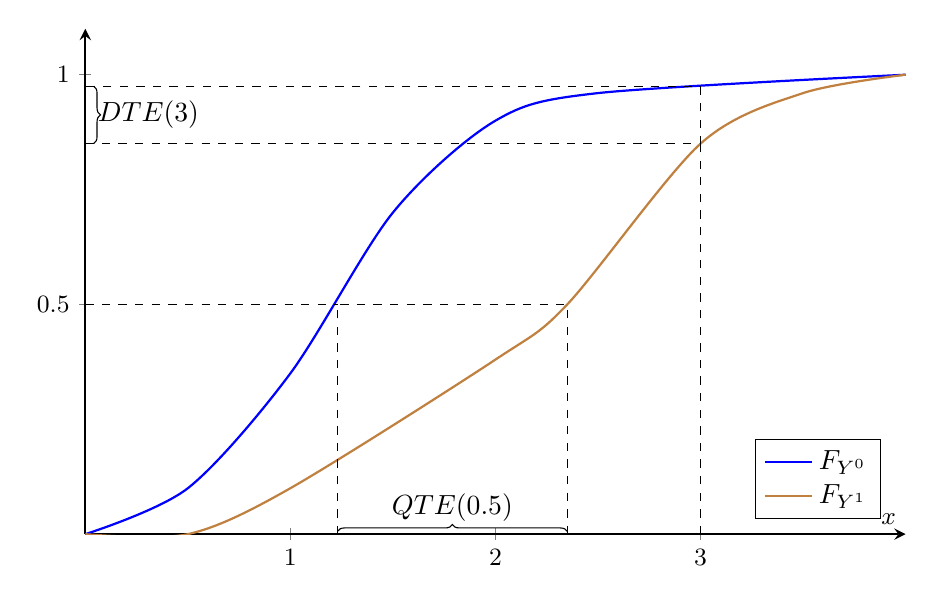
\begin{tikzpicture}
		
		% Define the axis and plot properties
		\begin{axis}[
			width=12cm, height=8cm,
			xmin=0, xmax=4,
			ymin=0, ymax=1.1,
			axis lines=middle,
			xlabel={$x$},
			ylabel={},
			xtick={0,1,2,3},
			ytick={0,0.5,1},
			legend pos=south east,
			tick label style={font=\small},
			label style={font=\small},
			axis line style={thick}
			]
			
			% Plot the first nonlinear CDF (blue)
			\addplot[
			thick,
			smooth,
			color=blue
			] coordinates {
				(0,0) (0.5,0.1) (1,0.35) (1.5,0.7) (2,0.9) (2.5,0.96) (4, 1)
			};
			\addlegendentry{$F_{Y^0}$}
			
			% Plot the second nonlinear CDF (red)
			\addplot[
			thick,
			smooth,
			color=brown
			] coordinates {
			(0, 0) (0.5, 0)	(1,0.1)   (2,0.38) (2.35, 0.5)   (3,0.85) (3.5,0.96) (4, 1)
			};
			\addlegendentry{$F_{Y^1}$}
			
			% Vertical dashed line for DTE
			\draw[dashed] (axis cs:0,0.85) -- (axis cs:3,0.85) -- (axis cs:3,0.975) -- (axis cs:0,0.975);
			
   			\draw[dashed] (axis cs:3,0)  -- (axis cs:3,0.85);			
 

				\draw[decoration={brace,mirror, raise=3pt},decorate]
			(axis cs: 0,0.85) -- node[right=1pt] {$DTE(3)$} (axis cs: 0, 0.975); 
			
						% Horizontal dashed line for QTE
			\draw[dashed] (axis cs:1.23,0) -- (axis cs:1.23,0.5) -- (axis cs:2.35,0.5) -- (axis cs:2.35,0);
			
			\draw[dashed] (axis cs:0,0.5)  -- (axis cs:1.23,0.5) ;
			
	  
			\draw[decoration={brace,raise=1pt},decorate]
			 (1.23,0) -- node[above=1pt] {$QTE(0.5)$} (2.35,0); 
			
		\end{axis}
		
	\end{tikzpicture}
	 \caption{Visual representation of distributional treatment effects (DTEs) and quantile treatement effects (QTEs).  Depicted: $DTE(3)$ --- difference of CDFs of potential outcomes distributions at $y=3$ and $QTE(0.5)$ --- difference of medians of potential outcome distributions}\label{quantile:figure:qte_dte} 
	 
	
\end{figure} 
 
 
   
 \paragraph{Interpretation of QTEs and DTEs}
 
 Are the DTEs and QTEs of any policy interest?  A typical interpretation under SUTVA goes as follows.   QTEs and DTEs express the distributional effects of making one of the treatment options universal. Under SUTVA, the resulting distribution of outcomes will be exactly given by the marginal distribution of the corresponding potential outcomes. The QTEs and the DTEs will contrast the distributions under these two alternative options. 
 
 Between the QTE and the DTE, the QTE is slightly easier to interpret, as QTEs are are expressed in terms of the outcome variable. In contrast, the DTEs are slightly more complicated to interpret, as they are expressed in terms of changes in CDFs.
 
 
 
 
 \paragraph{Conditional  or unconditional effects?}
 
 When non-treatment covariates $X_i$ are available, one must   choose whether the interest lies in quantiles that are conditional or unconditional given $X_i$.  In contrast to average effects, this choice leads to parameters that are not connected by integrating over $X_i$ and involve different identification arguments. 
 
To understand the practical difference, consider the following example.  Let $D_i$ be a job training program, $X_i$ be the person's education attainment, and $Y_i$ be earnings. The 10th percentile of the potential outcomes for \emph{college}-educated people may lie fairly high in the overall (marginal) distribution of outcomes.
 
 

\subsection{Regarding the Distribution of Treatment Effects}
  

  
  
 
\paragraph{DTEs and QTEs are not distributional features of treatment effects}

Importantly, the QTE is \emph{not} equal to the quantile of treatment effects outside of some special cases. Formally, it is usually the case that 
\begin{equation}
	 Q_{Y^{d'}}(\tau) - 	Q_{Y^d}(\tau)  \neq Q_{Y^{d'}- Y^d}(\tau).
\end{equation}
Similarly, the DTE in general is only loosely related to the distribution of treatment effects. 


 
\paragraph{Usually only partial identification for distribution of treatment effects}

The distribution of quantile effects is only partially identified even in  experimental settings (outside of very restrictive settings). Even the best experiments usually allow us to identify at most the marginal   distributions $F_{Y^1}$ and $F^{Y^0}$. Then at most the following can be said about the distribution  $F_{Y^1-Y^0}(\cdot)$ and the quantiles of treatment effects:
\begin{align}
	F^L(y) & \leq F_{Y^1-Y^0}(y)\leq F^U(y),\\
	Q^L(\tau) & \leq Q_{Y^1-Y^0}(\tau) \leq Q^U(\tau),
\end{align} 
for
\begin{align}
	F^L(y) & = \sup_w \max\curl*{(F_1(w) - F_0(w-y), 0},\\
	F^U(y) & = 1+ \inf_w\min\curl*{F_1(w) - F_0(w-y), 0 },\\
			Q^L(\tau) & = \sup_{w\in [0, \tau]}\left( F_X^{-1}(w) + F_Y^{-1}(\tau-w) \right), \\
			 Q^U(\tau) & = \inf_{w\in [\tau, 1]} \left(F_X^{-1}(w)  + F^{-1}_Y(1+\tau-w)\right). \\
\end{align} See   \cite{Makarov1981} and \cite{Williamson1990} regarding these bounds. They are known to be pointwise sharp. \cite{Fan2010} discuss inference on such bounds. See also \cite{Firpo2019} for some refinements.



\paragraph{Comonotonicity: when   QTEs  are the quantiles of the individual treatment effects}



QTEs do correspond to the quantile of the treatment effect in the special case of perfect rank correlation (comonotonicity, rank preservation) between potential outcomes \citep{Doksum1974EmpiricalProbabilityPlots}. Consider the case of a binary treatment $d=0, 1$. 
%
Comonotonicity means that the potential outcomes have the Skorokhod representation
\begin{equation}
	(Y^1_i, Y^0_i) = \left(F_{Y^1}^{-1}(U_i), F_{Y^0}^{-1}(U_i)\right).
\end{equation}
where $U_i$ is a common Uniform[0, 1] random variable. Intuitively, each individual has the same rank in all of the potential outcome distributions.
% 

In this special case it is indeed true that the difference in quantiles is equal to the quantile of the difference (the treatment effect). Moreover, the above representation also implies that the potential outcomes can be determined as 
\begin{equation}
	Y^1_i = F_{Y^1}^{-1}\left( F_{Y^0} (Y^0_i) \right).
\end{equation}
%Assume that the treatment effect of $D$ is entirely determined by the potential outcome $Y^0$ and equal to $\Delta(Y^0)$.  
%
%Further, suppose that $\Delta(\cdot)$ is such that $y+ \Delta(y)$ is non-decreasing.  If $F_{Y^0}$ is continuous, Then according to theorem 2.1 in \cite{Doksum1974EmpiricalProbabilityPlots} 
%\begin{equation}
%	F_{Y^0}(y) = F_{Y^1}(y+\Delta(y)).
%\end{equation}


% \paragraph{Quantiles or distributional? Computational connection}
% 
% 
% Does not matter which one you choose, since p. 2212 \cite{Chernozhukov2013b}
 \newpage 
 
  

\section{Nonparametric Identification of Distributions of Potential Outcomes Under Unconfoundedness}
 \label{quantile:section:identification_qtes_dtes_unconfounded} 
  
 We now turn to  identifying the quantile and distributional parameters discussed in section \ref{quantile:section:causal_background}.
%
For all of the parameters of interest,  it will be sufficient to identify the quantile or distribution functions of the potential outcomes. Accordingly, we will focus on these objects throughout.

In this section, we will consider identification  under unconfoundedness, while identification under endogeneity is deferred to section \ref{quantile:section:iv_qr}. As we will see, the identification argument will be similar for all of the parameters of interest.  

Our approach will be nonparametric. It will impose no functional form restrictions on potential outcomes or individual-level heterogeneity.

\subsection{Identification Under Unconditional Unconfoundedness (RCT)}

\paragraph{Setting with unconditional unconfoundedness}

We begin by considering the simplest setting in which the treatment $D_i$ is marginally independent from the collection of potential outcomes:
\begin{equation}\label{quantile:equation:unconditional_unconfoundedness}
	\curl{Y^d_i}_{d} \ind D_i.
\end{equation}  
There may potentially be some covariates $X_i$, which are marginally independent of $D_i$.

This setting is represented by the single-world intervention graph on fig. \ref{quantile:figure:qte_swig_2}. It corresponds to a randomized controlled trial where the treatment is assigned independently of potential outcomes and other individual characteristics  (a random effects setting).

 



\begin{figure}[ht!]
	
	  		\centering
	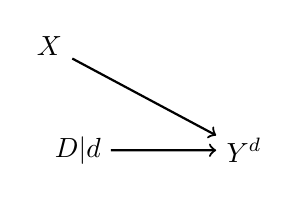
\begin{tikzpicture}[thick, scale=12]
		
		\node (v1) at (0.397,-0.432) {$D|d$};
		\node (v2) at (0.573,-0.432) {$Y^d$}; 
		\node (v3) at (0.367,-0.322) {$X$}; 
		\draw [->] (v1) -- (v2); 
		\draw [->] (v3) -- (v2);
	\end{tikzpicture}
	\caption{Representation of setting \eqref{quantile:equation:unconditional_unconfoundedness} (unconditional unconfoundedness)}\label{quantile:figure:qte_swig_2}
	
	
\end{figure}

As always, the realized outcome $Y_i$ will be equal to $Y^d_i$ if $D_i=d$. The treatment $D_i$ may be discrete- or continuous-valued. In the latter case, we implicitly assume all the regularity conditions which permit us to work conditionally on events of the form $\curl{D_i=d}$.

\paragraph{Objects of interest}

 
 In this setting, interest typically lies on the marginal (unconditional) distribution and quantiles of potential outcomes $Y^d$. If  $X_i$ is present, we may also be interested in the conditional distribution of potential outcomes. 
 Observe that there is no new parameter is gained by conditioning on values of $D_i$ --- unconditional unconfoundedness implies that $F_{Y^d|D}(\cdot|k) = F_{Y^d}(\cdot)$ for any $k$.

\paragraph{Identification of the CDF of potential outcomes}
 
 We begin with the CDF $F_{Y^d}(\cdot)$ of $Y^d_i$. Identification is constructive and follows the following chain of equalities:
\begin{align}
	F_{Y^d}(y) & = \E\left[ \I\curl{Y^d_i\leq y} \right] \\
	& = \E\left[ \I\curl{Y^d_i\leq y} |D_i=d \right]\\
	& = \E\left[ \I\curl{Y_i\leq y}|D_i=d \right]\\
	& = F_{Y|D}(y|d). 
\end{align}
Here we take two key steps. In the second equality, we use independence of $Y_i^d$ and $D_i$. In the third line, we use   that the realized outcome $Y_i$ is equal to $Y^d_i$ when $D_i=d$.


\paragraph{Identification of quantiles of potential outcomes}
 
 In order to identify the quantiles of potential outcomes, we will assume that the corresponding distribution functions are continuous and strictly increasing. By the arguments of section \ref{quantile:section:quantile_properties}, it follows that the $\tau$th quantile of potential outcomes is uniquely characterized by the following moment condition:
 \begin{equation}
  P\left(Y^d_i\leq  Q_{Y^d}(\tau)  \right) = 	 \tau  .
 \end{equation}
 We can now again apply a conditioning argument to the above moment:
\begin{align}
	\tau & = P\left(Y^d_i\leq  Q_{Y^d}(\tau)  \right) = \E\left[ \I\curl*{Y^d_i\leq Q_{Y^d}(\tau)} \right] \\
	& = \E\left[\I\curl*{Y^d_i\leq Q_{Y^d}(\tau) }  |D_i=d   \right]\\
	& = \E\left[\I\curl*{Y_i\leq Q_{Y^d}(\tau) }|D_i=d \right].
\end{align}
As with the CDF, the second line uses unconfoundedness, while third line follows by the definition of $Y_i$.

Under our continuity and monotonicity assumptions, we conclude that 
\begin{equation}
	 Q_{Y^d}(\tau) = Q_{Y|D}(\tau|d).
\end{equation} 
In other words, the $\tau$th quantile of $Y^d_i$ is exactly the $\tau$th quantile of the observed outcome $Y_i$ in the group with $D_i=d$. 
 
 
\paragraph{Identification of the conditional CDF}
 
 Identification of the conditional distribution and quantiles of potential outcomes is also straightforward. We only consider the CDF:
 \begin{align}
 	F_{Y^d|X}(y|x) & = \E\left[ \I\curl{Y^d_i\leq y}|X_i=x \right] \\
 	& = \E\left[ \I\curl{Y^d_i\leq y} |D_i=d, X_i=x \right]\\
 	& = \E\left[ \I\curl{Y_i\leq y}|D_i=d, X_i=x \right]\\
 	& = F_{Y|D, X}(y|d, x).
 \end{align}
  Here we use the independence of $D_i$ and $X_i$ in addition to the unconfoundedness condition \eqref{quantile:equation:unconditional_unconfoundedness}. The argument for the quantiles of $Y^d_i$ is analogous. 
   
   
  
 
 
 \subsection{Identification Under Conditional Unconfoundedness}
 
 
 
 
\paragraph{Setting with conditional unconfoundedness}
 
 In practice, it is more frequent to see an assumption of conditional unconfoundedness given some  covariates $X_i$:
\begin{equation}\label{quantile:equation:conditional_unconfoundedness}
 \curl{Y_i^d}_d \ind D_i|X_i.
\end{equation}
 This setting is depicted on fig. \ref{quantile:figure:qte_swig_conditional_unconfoundedness}. It may correspond both to observational and stratified experimental settings. 
 
 
 
  \begin{figure}[ht!]
 	
 	\centering
 	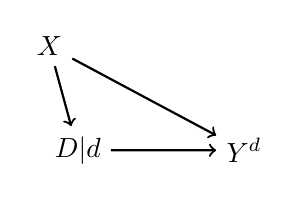
\begin{tikzpicture}[thick, scale=12]
 		
 		\node (v1) at (0.397,-0.432) {$D|d$};
 		\node (v2) at (0.573,-0.432) {$Y^d$}; 
 		\node (v3) at (0.367,-0.322) {$X$}; 
 		\draw [->] (v1) -- (v2); 
 		\draw [->] (v3) -- (v2);
 		\draw [->] (v3) -- (v1);
 	\end{tikzpicture}
 	\caption{Representation of setting \eqref{quantile:equation:conditional_unconfoundedness} (conditional unconfoundedness)}\label{quantile:figure:qte_swig_conditional_unconfoundedness}
 	
 	
 \end{figure}
 
 
 \paragraph{Objects of interest}
 
 Setting \eqref{quantile:equation:conditional_unconfoundedness} is fairly rich and allows us to consider both unconditional and conditional features.  We will focus on (in the order of identification):
 \begin{itemize}
 	\item Conditional quantiles and CDF of $Y^d_i$ given $X_i=x$;
 	\item Unconditional quantiles and CDF of $Y^d_i$;
 	\item Conditional quantiles of CDF of $Y^d_i$ given $D_i=k$.
 \end{itemize}
% Note that under conditional 
% here conditional on $(D_i, X_i)$ is equal to $X_i$ thanks to unconfoundedness
 
 \paragraph{Quantiles of potential outcomes given covariates}
  
  We begin with the simplest identification argument --- that of the conditional quantiles of $Y^d_i$ given $X_i=x$.   We will assume that the conditional CDF of $Y^d_i$ given $X_i=x$ is continuous and strictly increasing. Under these assumptions the conditional quantile $Q_{Y^d|X}(\tau|x)$ satisfies the moment condition
  \begin{equation}
P\left(Y^d_i \leq Q_{Y^d|X}(\tau|x)|X=x \right) =  \tau.
   \end{equation}
The left hand side of the moment condition can be represented exactly as before:
 \begin{align}
 	\tau & = P\left(Y^d_i \leq Q_{Y^d|X}(\tau|x)|X=x \right) = \E\left[ \I\curl*{ Y^d_i \leq Q_{Y^d|X}(\tau|x) } |X_i=x\right]\\
 	& =  \E\left[ \I\curl*{ Y^d_i \leq Q_{Y^d|X}(\tau|x) } |D_i=d, X_i=x\right]\\
 	& = \E\left[ \I\curl*{ Y_i \leq Q_{Y^d|X}(\tau|x) } |D_i=d, X_i=x\right],
 \end{align} 
 where we use conditional independence of $D_i$ and $Y_i^d$ in the second line and the definition of the observed outcome $Y_i$ in the third line.
 
 By continuity and strict monotonicity we conclude that 
 \begin{equation}\label{quantile:equation:conditional_potential_outcomes_quantile_idenfication}
 	 Q_{Y^d|X}(\tau|x) = Q_{Y|D, X}(\tau|d, x).
 \end{equation}
 In other words, the conditional quantile of potential outcome given covariates is equal to the conditional quantile of the observed outcomes given both covariates and the treatment. 
 
 
 
 
 \paragraph{Unconditional quantiles of potential outcomes: IPW representation}
 
 The argument for unconditional quantile $Q_{Y^d}(\tau)$ is more delicate. In contrast to average effects,  we cannot integrate eq. \eqref{quantile:equation:conditional_potential_outcomes_quantile_idenfication} with respect to the marginal distribution of $X$. 
 Instead, identifying $Q_{Y^d}(\tau)$ involves adapting the preceding approach to the unconditional case. 
We again start with the moment condition satisfied by the quantile of interest:
\begin{align}
	\tau & = P(Y^d_i\leq Q_{Y^d}(\tau) ) =  \E\left[ \I\curl{Y^d_i\leq Q_{Y^d}(\tau)  }\right] =  \E\left[ \E\left[ \I\curl{Y^d_i\leq  Q_{Y^d}(\tau)  }|X_i \right]  \right] \\
	& =   \E\left[ \E\left[\I\curl{Y^d_i\leq Q_{Y^d}(\tau)  }| D_i=d, X_i\right]\right]  \\
	& = \E\left[ \E\left[\I\curl{Y_i\leq Q_{Y^d}(\tau)  }| D_i=d, X_i\right]\right].
\end{align}
 Here we again use unconfoundedness and the definition of the observed again.
 
 The above expression is inconvenient, as it involves iterating an expectation. To obtain a simpler moment condition, we proceed as follows
 \begin{align}
 	&  \E\left[ \E\left[\I\curl{Y_i\leq Q_{Y^d}(\tau)  }| D_i=d, X_i\right]\right] \\
 	& =  \E\left[ \E\left[\I\curl{D_i=d}\I\curl{Y\leq Q_{Y^d}(\tau) }|D_i=d, X\right]\right]\\
 	& = \E\left[ \dfrac{1}{P\left(D_i=d|X_i\right)} \E[\curl{D_i=d} \I\curl{Y_i\leq  Q_{Y^d}(\tau) }|X] \right]\\
 	& =  \E\left[\E\left[  \dfrac{1}{P\left(D_i=d|X_i\right)} \I\curl{D_i=d} \I\curl{Y_i\leq  Q_{Y^d}(\tau) }|X\right] \right] \\
 	& = \E\left[  \dfrac{\I\curl{D_i=d} }{P\left(D_i=d|X_i\right)}\I\curl{Y_i\leq Q_{Y^d}(\tau) }\right].
 \end{align}
 Here
 \begin{itemize}
 	\item The first equality  uses that $D_i=d$ conditional on $\curl{D_i=d}$.
 	\item The second line uses the following version of the law of total expectations.  If $Z$ is a random variable and $T$ is a 0/1 random variable, 
 	\begin{equation}
 		\E[Z|X] =  P(T=1|X) \E[Z|X, T=1]  + (1-P(T=0|X)) \E[Z|X, T=0].
 	\end{equation}
 To apply it, take $T_i = \curl{D_i=d}$ and  $Z = T\I\curl{Y_i\leq Q_{Y^d}(\tau)}$.  The second term above is zero, and hence
 	\begin{align}
 & 		\E\left[\I\curl{D_i=d}\I\curl{Y\leq q_{1, \tau} }|D_i=d, X_i\right] 
 \\ 
 & = \dfrac{1}{P\left(D_i=d|X_i\right)} \E[\curl{D_i=d} \I\curl{Y_i\leq  Q_{Y^d}(\tau) }|X_i].
 	\end{align}
% 	\item The last line moves $1/p(X)$ into the conditional expectation and integrates over $X$ to move back to an unconditional expectation.
 \end{itemize}
 In summary, we have shown that the unconditional quantile of interest  $ Q_{Y^d}(\tau)$ satisfies the following moment condition:
 \begin{equation}
 	 \E\left[  \dfrac{\I\curl{D_i=d} }{P\left(D_i=d|X_i\right)}\I\curl{Y_i\leq Q_{Y^d}(\tau) }\right] = \tau.
 \end{equation}
  Intuitively, this moment conditions shows that $ Q_{Y^d}(\tau)$ is the $\tau$th quantile of a suitably reweighted distribution of the observed outcome. Weighting is done by the inverse of the propensity scores $P(D_i=d|X)$, and hence the above is an example of inverse probability weighting. 
 This argument is originally due to \cite{Firpo2007EfficientSemiparametricEstimation}.
   
   \paragraph{Quantiles of potential outcomes given $D_i$}
   
   A similar argument to the above one can be used to identify quantiles of the form $Q_{Y^d|D}(\tau|k)$.
   
%   \begin{align}
%   	\tau & =  P\left(Y^d_i \leq Q_{Y^d|D, X}(\tau|k, x)|D_i=k, X_i=x \right)\\
%   	&  = \E\left[ \I\curl*{Y^d_i \leq Q_{Y^d|D, X}(\tau|k, x)}| D_i=k, X_i=x \right]\\
%   	& = \E\left[ \I\curl*{Y^d_i \leq Q_{Y^d|D, X}(\tau|k, x)}| D_i=d, X_i=x \right]\\
%   	& = \E\left[ \I\curl*{Y_i \leq Q_{Y^d|D, X}(\tau|k, x)}| D_i=d, X_i=x \right]
%   	   \end{align}
%   	   
%   	   
%   The previous arguments can now be leveraged to obtain identification of quantiles of the form $Q_{Y^d|D}(\tau|k)$.  
 
\paragraph{CDF conditional on $X_i$}

The arguments for identifying the distribution functions of potential outcomes flow similarly to the ones for quantiles.  First, we consider the conditional CDF of $Y^d_i$ given $X_i=x$:
\begin{align}
	F_{Y^d|X}(y|x) & =\E\left[\I\curl{Y^d_i\leq y}|X_i=x \right]\\
	& = \E\left[\I\curl{Y^d_i\leq y}|D_i=d, X_i=x \right]\\
	& = \E\left[ \I\curl{Y_i\leq y}|D_i=d, X_i=x   \right]\\
	& = F_{Y|D, X}(y|d, x),
\end{align}
where we have again used unconfoundedness and the definition of $Y_i$.
In words, the CDF of interest is equal to a particular conditional distribution of the observed outcome $Y_i$.

\paragraph{Unconditional CDF of potential outcomes}

To identify the marginal CDF of $Y^d_i$, we adapt the above conditional argument and iterate expectations as follows:
\begin{align}
	F_{Y^d}(y) &  = \E\left[ \I\curl{Y^d_i \leq y} \right] = \E\left[ \E\left[ \I\curl{Y^d_i \leq y}|X_i \right]\right]\\
	& = \E\left[ \E\left[ \I\curl{Y^d_i \leq y}|D_i=d, X_i \right]\right]\\
	& = \E\left[ \E\left[ \I\curl*{Y_i\leq y}| D_i=d, X_i \right]  \right]\\
	& = \E\left[  F_{Y|D, X}(y|d, X_i) \right]\\
	& = \int F_{Y|D, X}(y|d, x)F_X(dx).
\end{align} 
The marginal CDF of interest is identified as a suitably reweighted conditional CDF of the observed outcome. Observe that the object in the last line is \emph{not} the same as $F_{Y|D}(y|d)$. 

Note that it is also possible to obtain an IPW expression for $F_{Y^d}(y)$ by proceeding as with $Q_{Y^d}$ starting from the iterated expectation. See \cite{Donald2014EstimationInferenceDistribution}.

\paragraph{CDF conditional on value of $D_i$}
 
Extending the above logic, we can also identify the conditional CDF $F_{Y^d|D}(y|k)$ through the following argument:
\begin{align}
	F_{Y^d|D}(y|k)  & =  \E\left[ \I\curl{Y^d_i \leq y}|D_i=k \right] = \E\left[ \E\left[ \I\curl{Y^d_i \leq y}|D_i=k, X_i \right]|D_i=k\right]\\
	& =  \E\left[ \E\left[ \I\curl{Y^d_i \leq y}|D_i=d, X_i \right]|D_i=k\right]\\
	& = \E\left[ \E\left[ \I\curl{Y_i\leq y}|D_i=d, X_i \right]|D_i=k\right]\\
	& = \E\left[ F_{Y|D, X}(y|d, X_i)|D_i=k \right]\\
	& = \int F_{Y|D, X}(y|d, x) F_{X|D}(dx|k). \label{quantile:equation:counterfactual_distribution}
\end{align}
In the last line we make an implicit assumption  that  the support of $X_i$ conditional on $D_i=k$ is included in the support of $X_i$ conditional on $D_i=d$. Without such an assumption the integral may not be well-defined. 

When $k=d$, the above argument simply reduces to 
\begin{equation}
	 F_{Y^d|D}(y|k) = F_{Y|D}(y|d).
\end{equation}

\paragraph{Aside: counterfactual distribution}

Objects of the form \eqref{quantile:equation:counterfactual_distribution} are sometimes called \emph{counterfactual distributions} in the literature \citep{Machado2005CounterfactualDecompositionChanges, Chernozhukov2013b}. In principle, they may be defined in any setting regardless of unconfoundedness, and can be used to do Oaxaca-Blinder-type decompositions. 
   
%
%\paragraph{unifying}
%
%\cite{Powell2020} discusses a matter of unifying all of these identification arguments, and also including potential identification under instrumental variables. 
 
  
\newpage 

\section{Estimation Methods: Quantile  Regression}
 
 \subsection{Towards Estimation}
 
 \paragraph{Common identification feature: conditional distributions of $Y_i$}
 
 A common theme in the identification results of the previous section is that we express the parameters of interest in terms of conditional distribution or quantiles of the observed outcome $Y_i$.  Hence, it is sufficient to estimate these quantities to estimate the objects of interest. 
  

\paragraph{Estimation with discrete-only covariates}

It is easy to estimate the required CDFs/quantiles of $Y_i$ when the conditioning variables are discrete. In this case splitting the sample and focusing on the corresponding subsample is sufficient.   The empirical distribution function of $Y_i$ in the subsample serves as an estimator for the conditional CDF. The quantiles of $Y_i$ can be estimated with sample quantiles.

\paragraph{Estimation in more general cases: quantile and distribution regression}

Splitting the sample is not feasible if there are continuously-distributed conditioning variables present.   In this case, one has to approximate the quantiles or the CDF. \emph{Quantile} and \emph{distribution regression} are two methods methods for estimating the parameters of such approximations:
\begin{itemize}
	\item Quantile regression directly models conditional quantiles of the type $Q_{Y|X}$.
	\item Distribution regression instead models conditional distribution function $F_{Y|X}$.
\end{itemize} 
In this section, we first given a general introduction to these methods, and then apply them to estimating the causal parameters of interest. 

\subsection{Introduction to Quantile Regression}



\paragraph{Setting}

We now give a brief introduction to quantile regression, temporarily disregarding our causal framework.  For further information, see the monograph by \cite{Koenker2005} and the Handbook of Quantile Regression \citep{Koenker2017HandbookQuantileRegression}.

Let $Y_i$ be some outcome variable and $X_i$ be a vector of covariates.  The conditional CDF $F_{Y|X}(\cdot|x)$ is assumed to be continuous and strictly increasing for all $x$. We observe a IID sample $\curl{Y_i, X_i}_{i=1}^N$. 
  
\paragraph{Population nonparametric quantile regression}


Interest lies in the estimating the $\tau$th quantile $Q_{Y|X}(\tau|x)$ of $Y_i$ given on $X_i=x$.  We do not assign any causal interpretation to this quantile.

The parting point for all of quantile regression is representation \eqref{quantile:equation:conditional_quantile_unconditional_minimizer}. Under the assumptions on the CDF of $Y_i$, this representation  shows that that   $Q_{Y|X}(\tau|x)$  uniquely minimizes the check risk: 
\begin{equation}\label{quantile:equation:quantile_regression_minimizer_representation}
	Q_{Y|X}(\tau|X)  =  \argmin_{q(X)}  \E[\rho_{\tau}(Y-q(X))],
\end{equation}
where the minimum is taken over the class of all measurable functions. 


\paragraph{Infeasibility of the population problem}

The above characterization is not directly useful for two familiar reasons:
\begin{itemize}
	\item The check risk in \eqref{quantile:equation:quantile_regression_minimizer_representation} is a population quantity, while we only have access to a finite sample in practice. 
	\item The class of all measurable functions is too large to search through unless the support of $X$ is finite. 
\end{itemize}
%The development will be similar to linear regression (similarity are not accidental, as \textcolor{red}{TBA} \cite{Angrist2006QuantileRegressionMisspecification}	show).

\paragraph{Sample objective function}

We deal with the first problem by replacing the population expectation with a sample one to obtain the sample objective function:
\begin{equation}
	 \E_N[\rho_{\tau}(Y-q(X))] \equiv \dfrac{1}{N} \sum_{i=1}^N \rho_{\tau} (Y_i - q(X_i)). 
\end{equation}


\paragraph{Functional form choice for quantile, linear specification}
 
To deal with the second problem, we restrict $q(\cdot)$ to a simpler space, typically finite-dimensional. 
The simplest and most popular approach restricts $q(\cdot)$ to be linear in parameters:
\begin{equation}
	q(x, \beta) = \psi(x)'\beta,
\end{equation}
where $\psi(\cdot)$ is some known transformation of covariates (e.g. polynomials, interactions).
%

Such a model can be assume to hold only for one $\tau$, or for a range of $\tau$. In the latter case, the coefficient vector is allowed to be $\tau$-specific:
\begin{equation}\label{causal:equation:linear_quantile_specific}
	q(x, \beta(\tau)) = \psi(x)'\beta(\tau). 
\end{equation}

\paragraph{Fitting quantile regression}

After specifying some form for the conditional quantiles, the resulting parameters are then estimated by minimizing the sample objective function for each $\tau$ of interest.

 For example, in the linear case the parameters are estimated as in the canonical quantile regression of \cite{Koenker1978RegressionQuantiles}
\begin{equation}
	\hat{\beta}(\tau)= \argmin_{b} \dfrac{1}{N}\sum_{i=1}^N \rho_{\tau}(Y_i-\psi(X_i)'b)
\end{equation} 
If $q(\cdot)$ is linear in parameters, the above problem can be represented as a linear optimization problem and solved quickly even for large $N$; see \cite{Koenker2017ComputationalMethodsQuantile} regarding the computational aspects of the above minimization problem.


The resulting estimator for conditional quantiles is given by
\begin{equation}
	 \hat{Q}_{Y|X}(\tau|x) = \psi(x)'\hat{\beta}(\tau).
\end{equation}



\paragraph{Regarding specification: parametric vs. nonparametric approaches}

%Note that this section is deliberately vague about whether this   choice is just an approximation or an assumption of true functional form.
 
 As with mean regression, there are two perspectives on the choice of functional form:
\begin{itemize}
	\item \emph{Parametric}. In a parametric setting, we fix a given finite-dimensional class  for $q(\cdot)$, such as linear functions.
If the model is correctly specified, quantile regression will consistently estimate the true $Q_{Y|X}(\tau|x)$. 
If the choice is misspecified, quantile regression will estimate a particular ``best'' approximation  to the true $Q_{Y|X}(\tau|x)$, see 	 \cite{Angrist2006QuantileRegressionMisspecification}. Specification testing can be done using the methods of \cite{Rothe2013MisspecificationTestingClass}.
	\item \emph{Nonparametric}. In a nonparametric approach, $q(\cdot)$ is a flexible approximation that grows in complexity with $N$. Different approaches have been explored in the literature, including local polynomials, splines, random forests. See
	\cite{Koenker1994QuantileSmoothingSplines}, ch. 7 in \cite{Koenker2005},
	\cite{Meinshausen2006QuantileRegressionForests}, etc. As $N$ grows, quantile regression will consistently estimate $Q_{Y|X}(\tau|x)$ under mild conditions. 
	
\end{itemize}
  Asymptotic properties of the estimators can be established pointwise or uniformly in $\tau$, see \citep{Angrist2006QuantileRegressionMisspecification} for some general theory in the parametric case.
   

\subsection{When Is the Linear Model Correctly Specified?}

Before continuing the general discussion, we make a small detour to discuss the conditions under which \eqref{causal:equation:linear_quantile_specific} is correctly specified.

% two aspects of the linear conditional quantile model \eqref{causal:equation:linear_quantile_specific}:
%\begin{itemize}
%	\item The conditions under which 
%	\item The behavior of the linear index $\psi(x)'\beta(\tau)$ as a function of $x$ and $\tau$, and the question of quantile crossing.
%%	\item 
%\end{itemize}

\paragraph{When is the linear model correctly specified?}
 
% When is linear approximation \eqref{causal:equation:linear_quantile_specific} correctly specified?  
 To find such conditions, we go back to the conditional quantile transform \eqref{quantile:equation:skorokhod_conditional}.  
 %
 Let the conditional $\tau$th quantile of $Y_i$ given $X_i=x$ be given by $\psi(x)'\beta(\tau)$. Let $U_i$ be a Uniform[0, 1] random variable that is independent of $X$. Then eq. \eqref{quantile:equation:skorokhod_conditional} shows that $Y_i$ can be   generated as 
 \begin{equation}\label{quantile:equation:rct_quantile_representation}
 	 Y_i = Q_{Y|X}(U|X) = \psi(X_i)'\beta(U_i),
 \end{equation}  
 In other words, the linear quantile model  \eqref{causal:equation:linear_quantile_specific} is correctly specified if $Y$ follows a particular random coefficient model.
 
  Model \eqref{quantile:equation:rct_quantile_representation} is quite restrictive. All of the variation in the coefficients  $\beta(U_i)$ is due to the scalar source $U_i$. There is no independent variation between the coordinates of $\beta(U_i)$. In addition, the coefficients $\beta(U_i)$ are independent from the covariates $X_i$.
 
  \paragraph{Contrast with more general random coefficient models}
 
 It is worth contrasting   model \eqref{quantile:equation:rct_quantile_representation} with the random coefficient model considered by  \cite{Hoderlein2010}. \cite{Hoderlein2010} consider a more general random coefficient model of the form
 \begin{equation}\label{quantile:equation:rcm_hoderlein_et_al}
 	Y_i = \psi(X_i)'\beta_i,
 \end{equation} 
 where $\beta_i$ is independent from $X_i$. Model \eqref{quantile:equation:rcm_hoderlein_et_al} does not restrict the variation between the components of $\beta_i$.
 
  The key difference between   models \eqref{quantile:equation:rct_quantile_representation} and \eqref{quantile:equation:rcm_hoderlein_et_al} are the conditions under which they allow the distribution of $\beta_i$ to be identified.
 \begin{itemize}
 	\item  Model \eqref{quantile:equation:rcm_hoderlein_et_al} does not restrict variation in the coefficients. However, the vector $\psi(X_i)$ must have a ``full'' support in the sense that the density of $\psi(X_i)/\norm{\psi(X_i)}$ is supported on the whole unit sphere.
 	
 	
 	  Such an assumption rules out discrete covariates, polynomial and other functionally dependent components in $\psi(\cdot)$. It also complicates including an intercept term, though \cite{Hoderlein2010} explicitly address this case.
 	
 	\item   Model \eqref{quantile:equation:rct_quantile_representation} does not restrict  the regressors $\psi(X_i)$ beyond no multicollinearity. However, it   restricts independent variation between coefficients. 
 	 \end{itemize}
 
 


 
	 \subsection{Nonmonotonicity in Estimates of Quantiles and Rearrangement}

  Two important related issues affect quantile regression --- nonmotonicity and quantile crossing, see section 2.5 in \cite{Koenker2005}. These issues affect both parametric and nonparametric estimators, and may even manifest in populations. 

\paragraph{Monotonicity and the no-crossing properties}

As above, let $Q_{Y|X}(\tau|x)$ be the true $\tau$th quantile of $Y_i$ given $X_i=x$.

 As a quantile function, $Q_{Y|X}$ satisfies the properties of  monotonicity and non-crossing. These properties concern $Q_{Y|X}(\tau|x)$ as a function of $\tau$ and $x$, respectively:
 \begin{enumerate}
 	\item Monotonicity refers to the fact that the function $\tau\to Q_{Y|X}(\tau|x)$ must be non-decreasing in $\tau$ for every $x$.
 	
 	\item Non-crossing states that the functions  $x \to Q_{Y|X}(\tau|x)$ and $x\to Q_{Y|X}(\tau'|x)$ cannot cross unless $\tau=\tau'$. 
 	Formally, define the following family of functions indexed by $\tau$:
 	 \begin{equation}
 		\Fcal= 	\curl{ f_{\tau}: f_{\tau}(x)= Q_{Y|X}(\tau|x), \quad \tau\in (0, 1)}.
 	\end{equation} 
 The no-crossing property of $\Fcal$ is that  for no $x, x'\in \supp(X_i)$ and $\tau, \tau', \tau\neq\tau'$ may it be the case that 
 	\begin{equation}
 		f_{\tau'}(x)>f_{\tau}(x)  \quad f_{\tau'}(x)< f_{\tau}(x).
 	\end{equation}
 	The no-crossing property is a direct consequence of the monotonicity property.
 \end{enumerate}
%Both the non-

\paragraph{Violation of monotonicity and no-crossing (sample and population)}
 
 Recall that  estimating $Q_{Y|X}(\tau|x)$ by quantile regression involves three key steps: specifying some  tractable model $q(x, \beta(\tau))$ for $Q_{Y|X}(\tau|x)$; obtaining  a finite sample of data on $(Y_i, X_i)$; and estimating the parameters $\beta(\tau)$, separately for each $\tau$.
 
All three of the above steps can lead to non-monotonic and crossing estimates for the quantile function \citep{Bassett1982EmpiricalQuantileFunction}. Fig. 2.8 in \cite{Koenker2005} offers a typical example. As a consequence, the resulting estimates are not valid quantile functions, nor do they yield valid CDFs when inverted. 


 

  
\paragraph{Example of nonmonotonicity and crossing in population: linear models}
   
   Non-monotonicity and crossing may also manifest in population, depending on the model $q(x, \beta(\tau))$ and the support of data.  
   For example, a linear specification for $q(\cdot, \cdot)$ will display crossing, unless all the coefficients are independent from $\tau$.
   
   As a specific example, suppose that $X_i$ is scalar. Consider the situation depicted on fig. \ref{quantile:figure:quantile_crossing}, where we plot two lines that correspond to models for the $\tau$th and the $\tau'$th quantiles, respectively.
   The two lines necessarily cross, as  the slopes of the lines are different.
   
   If $X_i\in [4, 10]$, then the two lines on  \ref{quantile:figure:quantile_crossing} could be valid quantiles with $\tau'>\tau$. The opposite holds if $X\in [0, 2]$.  However, if the support of $X_i$ includes the interval $[2, 4]$, the two lines cannot be valid quantiles. If the linear approximation is used regardless, then non-monotonicity also holds in population. 
   
 
 \begin{figure}[ht!]
 	\centering
 	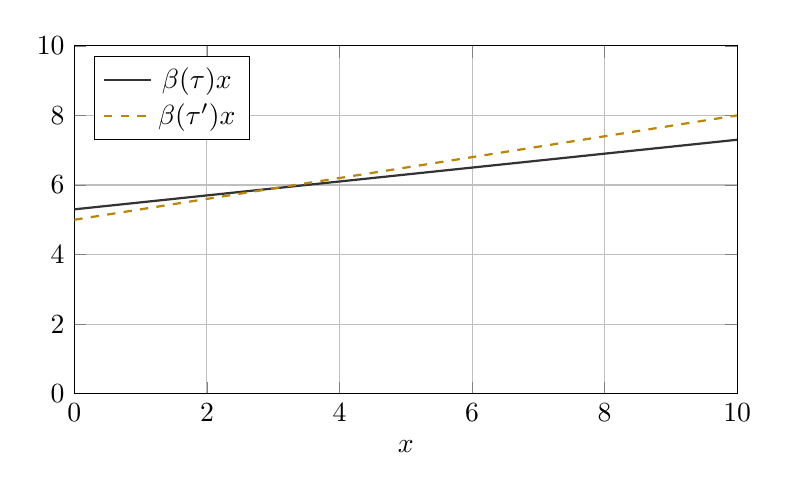
\begin{tikzpicture}
 		\begin{axis}[
 			width=10cm,
 			height=6cm,
 			xlabel={$x$},
 			ylabel={},
 			xmin=0, xmax=10,
 			ymin=0, ymax=10,
 			legend pos=north west,
 			grid=major,
 			xtick={0,2,...,10},
 			ytick={0,2,...,10},
 			]
 			
% 			% 25th percentile (red, dashed)
% 			\addplot [
% 			domain=0:10,
% 			samples=100,
% 			color=red,
% 			dashed,
% 			thick
% 			] {5 - 0.5 * x};
% 			\addlegendentry{25th percentile}
 			
 			% 50th percentile (blue, solid)
 			\addplot [
 			domain=0:10,
 			samples=100,
 			color=black!80,
 			thick
 			] {5.3 + 0.2 * x};
 			\addlegendentry{$\beta(\tau)x$}
 			
 			% 75th percentile (green, dotted)
 			\addplot [
 			domain=0:10,
 			samples=100,
 			color=DarkGoldenrod,
 			dotted,
 			dashed,
 			thick
 			] {5 + 0.3 * x};
 			\addlegendentry{$\beta(\tau')x$}
 			
 			% Highlight the crossing points
% 			\addplot [only marks, mark=o, color=black] coordinates {
% 				(5, 2.5)
% 				(5, 7.5)
% 			};
 			
 		\end{axis}
 	\end{tikzpicture}
 	 \caption{Example of quantile crossing}\label{quantile:figure:quantile_crossing}
 	 \end{figure}
 	  
   
 	  
 	  
 	 	 
 	 
 	    	
 	    	\paragraph{Rearrangement: solving non-monotonicity}
 	    	
 	    		 \emph{Rearrangement} offers a generic and attractive solution to the issue of non-monotonicity. It may be used with any quantile estimator. Rearrangement can also be used in other contexts where the target functions is monotonic. 
 	    	Its statistical properties were developed primarily by \cite{Chernozhukov2010QuantileProbabilityCurves}. 
 	    	
 	    	Rearrangement works as follows. Suppose that the $Q_{Y|X}(\tau|x)$ is modeled with some specification $q(x, \beta(\tau))$. Suppose that $\hat{\beta}(\tau)$ are the estimated coefficient of the model.  
 	    	Consider the random variable
 	    	\begin{equation}
 	    		\hat{W} = q(x, \hat{\beta}(U)), \quad U\sim\text{Uniform}[0, 1].
 	    	\end{equation}
     		
     	
 	    	The rearranged quantile function estimator is given by $\tau\to Q_{\hat{W}|X}(\tau|x)$ of $\hat{W}$.  Fig. \eqref{quantile:figure:rearrangement} provides a graphical example.
 	    	Note that if $q(x, \hat{\beta}(\tau))$ is non-decreasing in $\tau$, rearrangement leaves it unchanged.
 	    	
 	    	\paragraph{Rearranged CDF estimator}
 	    	
 	    	The monotonized estimator for the CDF is given by the CDF of $\hat{W}$, which can be obtained as 
 	    	\begin{equation}
 	    		\hat{F}(y|x) = \int_0^1 \I\curl{q(x, \hat{\beta}(\tau))\leq y }d\tau.
 	    	\end{equation}
% 	    	$\hat{Q}^*(u|x)$ is the quantile function of the CDF. In case the original quantile estimator is monotonic, the rearranged version is identical to it.
 	    	
 	    	\paragraph{Quantile bootstrap interpretation}
 	    	
 	    	$Q_{\hat{W}|X}(\tau|x)$ may be viewed as a bootstrap estimator --- specifically a form of parametric quantile bootstrap. 
 	    	
 	    	
 	    	\begin{figure}[ht!]
 	    		
 	    		\centering
 	    		
 	    		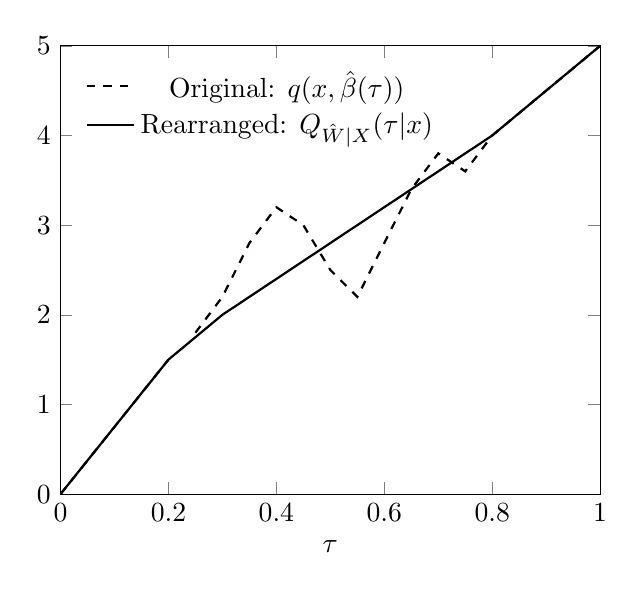
\begin{tikzpicture}
 	    			\begin{axis}[
 	    				xlabel={$\tau$},
 	    				ylabel={},
 	    				ymin=0, ymax=5,
 	    				xmin=0, xmax=1,
 	    				legend pos=north west,
 	    				legend style={draw=none}
 	    				]
 	    				% First curve: Q (dashed)
 	    				\addplot[dashed, thick] coordinates {
 	    					(0,0) 
 	    					(0.2,1.5)
 	    					(0.2,1.5)
 	    					
 	    					% Sinusoidal wave points between (0.2, 1.5) and (0.8, 4)
 	    					% Sinusoidal wave points with more oscillations
 	    					(0.25, 1.8)
 	    					(0.3, 2.2)
 	    					(0.35, 2.8)
 	    					(0.4, 3.2)
 	    					(0.45, 3.0)
 	    					(0.5, 2.5)
 	    					(0.55, 2.2)
 	    					(0.6, 2.8)
 	    					(0.65, 3.4)
 	    					(0.7, 3.8)
 	    					(0.75, 3.6)
 	    					(0.8,4) 
 	    					(1.0,5.0)
 	    				};
 	    				\addlegendentry{Original: $q(x, \hat{\beta}(\tau))$}
 	    				
 	    				% Second curve: Q* (solid)
 	    				\addplot[thick] coordinates {
 	    					(0,0) 
 	    					(0.2,1.5)
 	    					(0.2,1.5)
 	    					(0.3,2.0)
 	    					(0.4,2.4)
 	    					(0.5,2.8)
 	    					(0.6,3.2)
 	    					(0.7,3.6)
 	    					(0.8, 4)
 	    					(0.8,4) 
 	    					(1.0,5.0)
 	    				};
 	    				\addlegendentry{Rearranged: $Q_{\hat{W}|X}(\tau|x)$}
 	    			\end{axis}
 	    		\end{tikzpicture}
 	    		
 	    		\caption{Illustration: original non-monotonic estimator $q(x, \hat{\beta}(\tau))$ and the rearranged monotonic estimator $Q_{\hat{W}|X}(\tau|x)$}\label{quantile:figure:rearrangement}
 	    	\end{figure}
 	    	
% 	    	\paragraph{Computation on the grid}
% 	    	
% 	    	It is possible to compute the rearrangement by sorting on a finite fine grid of values. Let $\curl{u_1, \dots, u_k}$ be a fine grid in $(0, 1)$. Then let $\hat{Q}^*(u|x)$ be the $u$th quantile of $\curl{\hat{Q}(u_1|x), \dots, \hat{Q}(u_k|x)}$.
% 	    	
 	     
 	    	
 	    	\paragraph{Rearrangement improves estimation quality in all $L^p$ norms}
 	    	 
 	    	As it turns out, it is always good to apply rearrangement if measure the quality of estimation of $Q_{Y|X}(\cdot|x)$ in terms of any $L^p$ norm. Specifically, \cite{Chernozhukov2010QuantileProbabilityCurves} show that for any $p\in [1, \infty]$ it holds that
 	    	\begin{equation}
 	    		\norm{Q_{\hat{W}|X}(\cdot|x)-Q_{Y|X}(\cdot|x)}_p\leq \norm{ q(x, \hat{\beta}(\tau))-Q_{Y|X}(\cdot|x)}_{p}.
 	    	\end{equation}
     	\cite{Chernozhukov2010QuantileProbabilityCurves} also show that rearranged estimators enjoy the same asymptotic properties as the original estimators do. Consequently,  rearrangement also is not problematic for inference.
% 	    	In other words, the rearranged estimators should be preferred to the original ones.
% 	    	  Rearrangement is \href{https://rdrr.io/cran/quantreg/man/rearrange.html}{implemented} in the \texttt{quantreg} package in R.
 	    	
 	    	
  
 
% Note that rearrangement can be principle even applied in populations. It may be the same the the population counterpart is misspecified. 
   
   
%   \paragraph{Implementation}
 
% 
% 
% \paragraph{Properties of the linear index: monotonicity in model \eqref{quantile:equation:rct_quantile_representation}}
% 
% We now  take a   deeper look at the single index $\psi(x)'\beta(\tau)$ under an assumption of correct specification. For simplicity, we take $\psi(x)=x$ and assume that 
% \begin{equation}
% 	Q_{Y|X}(\tau|x) = x'\beta(\tau), \quad \forall \tau\in (0, 1), x.
% \end{equation}
% We first consider $x'\beta(\tau)$ as a function of $\tau$, and then as a function of $x$.
% 
% The index $x'\beta(\tau)$ in  model \eqref{quantile:equation:rct_quantile_representation} is necessarily monotonically increasing in $\tau$. This monotonicity is a consequence of the monotonicity property of quantiles (result \ref{quantile:theorem:basic_properties}).
% 
% Note, however, that the individual   coordinates of $\beta(\tau)$ do not have to be monotonic functions of $\tau$. However,  it is possible to reparametrize the model to ensure monotonicity in each coefficient, as section 2.6 in \cite{Koenker2005} describes. 
 
 
 \subsection{Introduction to Distribution Regression}
 \label{quantile:subsection:distribution_regression}
 
 \paragraph{Setting}
 
 While quantile regression serves to model conditional quantiles, distribution regression is used to model conditional distributions. The idea is originally due to  \cite{Foresi1995ConditionalDistributionExcess} and developed deeply by \cite{Chernozhukov2013b}.
 
 The parameter of interest is the conditional distribution function $F_{Y|X}(y|x)$. We will keep the argument $y$ fixed, analogously to keeping $\tau$ fixed in quantile regression. 
 
 \paragraph{Motivation: likelihood characterization of object of interest}
 
 To motivate distribution regression, we begin with the observation that the $F_{Y|X}(y|x)$ trivially satisfies the following moment condition:
 \begin{equation}
 	 \E\left[ \curl{Y_i\leq y}|X_i =x \right]=  F_{Y|X}(y|x).
 \end{equation}
 Distribution regression starts by viewing the above moment as a likelihood model for the binary variable $Z_i= \I\curl{Y_i\leq y}$. Conditionally on $X_i=x$, the distribution $Z_i$ satisfies
 \begin{equation}
 	 Z_i = \begin{cases}
 	   1, & \text{ with probability } F_{Y|X}(y|x),\\
 	   0, & \text{ with probability } 1- F_{Y|X}(y|x).
 	 \end{cases} 
 \end{equation}
 The corresponding likelihood function of the sample  $\curl{Z_i, X_i}_{i=1}^N$  is simply given by
 \begin{equation}\label{quantile:equation:dr_nonparametric_likelihood}
 	 L =  \prod_{i=1}^N \left(F_{Y|X}(y|X_i) \right)^{Z_i} \left(  1-F_{Y|X}(y|X_i)  \right)^{1-Z_i}.
 \end{equation}
 
 \paragraph{Issue: too much flexibility}
 
 Directly maximizing \eqref{quantile:equation:dr_nonparametric_likelihood} with respect to $F_{Y|X}(y|\cdot)$ will generally return an infinite number of solutions that are meaningfully different. They key reason is that likelihood \eqref{quantile:equation:dr_nonparametric_likelihood} at best pins down the values of $F_{Y|X}(y|\cdot)$ at the sample points $(X_1, \dots, X_N)$.
 
 \paragraph{Specifying a model for $F_{Y|X}(y|\cdot)$}
 
 The solution to the above indeterminacy is to specify a finite-dimensional model for $F_{Y|X}(y|x)$. The standard approach is to specify a  generalized linear model of the form
 \begin{equation}\label{quantile:equation:dr_specification}
 	F_{Y|X}(y|x) = \Lambda(\psi(x)'\beta(y)),
 \end{equation}
 where $\psi(\cdot)$ are some known transformations of $x$; the coefficients $\beta(y)$ are $y$-specific, and $\Lambda(\cdot)$ is some known link function (logit, probit, linear, etc).  As before, this model can be viewed parametrically or nonparametrically.
 
 
 \paragraph{Estimating parameters $\beta(y)$}
 
 The parameters $\beta(y)$ can be straightforwardly by maximizing the likelihood \eqref{quantile:equation:dr_nonparametric_likelihood} after inserting model \eqref{quantile:equation:dr_specification} for $F_{Y|X}(y|\cdot)$. Specifically,  the estimator satisfies
  \begin{equation}
 	\hat{\beta}(y) \in \argmax_b \sum_{i=1}^{N}\left[ \I\curl{Y_{i}\leq y} \ln \Lambda(\psi(X_{i})'b) + \I\curl{Y_{i}>y}\ln\left[1-\Lambda\left(\psi(X_{i}'b) \right) \right] \right].
 \end{equation} 
 If the likelihood is strictly concave, $\hat{\beta}(y)$ will be uniquely determined and easy to compute. Concavity will hold for a logistic and other standard link functions.
 
 The resulting estimator for $F_{Y|X}(y|\cdot)$ is given by
 \begin{equation}\label{quantile:equation:dr_estimator}
 	\hat{F}_{Y|X}(y|x)  = \Lambda\left(\psi(x)'\hat{\beta}(y) \right).
 \end{equation}  
 Distribution regression may be viewed as a continuum of binary regressions indexed by $y$.
 
 \paragraph{Issue of non-monotonicity}
 
 Like quantile regression, the distribution regression estimator \eqref{quantile:equation:dr_estimator} may suffer from a non-monotonicity (crossing) issue even under correct specification. Since $\hat{\beta}(y)$ are estimated separately for each $y$, it is possible that $\hat{F}_{Y|X}(y|x)$ is not a monotonic function of $y$. 
 
 A practical consequence of non-monotonicity is that a non-monotonic $\hat{F}_{Y|X}(y|x)$   cannot be inverted to obtain estimated quantiles.
 
  Luckily, this   issue can also be    resolved by rearrangment \citep{Chernozhukov2010QuantileProbabilityCurves, Chernozhukov2013b}.
 
 \paragraph{Contrast between distribution and quantile regression}
 
 	Both quantile and distribution regression are flexible methods for modeling conditional distributions. By specifying a sufficiently rich $\psi(x)$, both approaches can approximate conditional quantiles or CDF arbitrarily well.  Since quantiles and CDFs are linked through the definitions of quantiles and formula, the two methods will be equivalent in the limit.
 	
 	However, there are some differences between the two approaches (see 3.1.3 in \cite{Chernozhukov2013b}):
 	\begin{itemize}
 		\item Distribution regression is more flexible in terms of the distribution of $Y$. It easily accommodates discrete, continuous, or mixed $Y_i$. 
 		
 		In contrast, quantile regression may not be flexible if $Y_i$ is not distributed continuously.
 		
 		\item Both methods can be used to estimate both quantiles and distribution functions. However, the results will usually be numerically different outside of the setting where $\psi(x)$  is ``saturated'' (contains indicators for all points in the support of $X_i$ for discrete-valued $X_i$).
 	\end{itemize}
 	
 	
 	
 
 \subsection{Estimation of Quantiles and Distributions of Potential Outcomes}
 
 We are now in position to provide straightforward estimators for distributions and quantiles of potential outcomes under unconfoundedness. In all cases, the estimators will be based on the identifying expressions of section   \ref{quantile:section:identification_qtes_dtes_unconfounded}.
 
 \paragraph{Difference in approaches: $D_i$ discrete vs. $D_i$ continuous}
 
 Estimation approaches differ depending on whether the treatment $D_i$ is discretely or continuously distributed. Suppose that interest lies in the 
 conditional quantiles $Q_{Y|D, \dots}(\tau|d, \dots)$ or the conditional CDF $F_{Y|D, \dots}(y|d, \dots)$.
 \begin{itemize}
 	\item If $D_i$ is continuously distributed, it is simply treated as a covariate in quantile/distribution regression. 
 	
 	\item If $D_i$ is discretely distributed, there are two closely related approaches:
 	\begin{enumerate}
 		\item Restricting the sample to the observations with $D_i=d$. 
 		
 		\item Taking $D_i$ to be part of the covariate vector and including interactions of $D_i$ with other covariates. 
 		
 	\end{enumerate}
 	
 	 
 	 
 \end{itemize}
  
  
  \paragraph{Estimation under unconditional unconfoundedness}
  
  
  We begin by considering  estimation under unconditional unconfoundedness.  Recall that interest lies in estimating $F_{Y^d}(d)$, $Q_{Y^d}(\tau)$, $F_{Y^d|X}(y|x)$, and $Q_{Y^d|X}(y|x)$.
   
   The marginal CDF and quantiles are the easiest parameters to estimate. However, the estimation procedure differs depending on the nature of $D_i$, as described above:
   \begin{enumerate}
   	\item If $D_i$ has finite support, $F_{Y^d}(y)$ is consistently estimated by the empirical distribution function of $Y_i$ in the subsample with $D_i=d$.
   	
   	Similarly, $Q_{Y^d}(\tau)$ is consistently estimated by the sample $\tau$th quantile of $Y_i$ in the subsample with $D_i=d$.
   	
   	
   	\item If $D_i$ is continuously distributed, $F_{Y^d}(y)$ can be consistently estimated in two steps. First, run a distribution regression of $Y_i$ on a suitable vector $\psi(D_i)$. Second, evaluate the resulting estimator at $\psi(d)$.
   \end{enumerate}
The conditional CDF and quantiles given $X_i$ can be estimated similarly. If $D_i$ has finite support, one simply runs a quantile/distribution regression of $Y_i$ on  some $\psi(X_i)$ in the subsample with $D_i=d$. If $D_i$ is continuously distributed, $Y_i$ is regressed on an appropriate $\psi(D_i, X_i)$. 
   
  
  \paragraph{Estimation of conditional quantiles and CDF under conditional unconfoundeness}
  
  The above logic can be generalized to the case where only conditional unconfoundedness holds.   For simplicity, we will assume for the remainder that the support of $D_i$ is finite. 
  
  The conditional quantiles $Q_{Y^d|X}(\tau|x)$ and CDF $F_{Y^d|X}(y|x)$ can be estimated by straightforward quantile regression of $Y_i$ on $\psi(X_i)$ in the subsample with $D_i=d$.
 
 \paragraph{Estimation of unconditional quantiles under conditional unconfoundedness}
 
 The matter is slightly more delicate when estimating the unconditional quantiles $Q_{Y^d}(\tau)$ of potential outcomes. Recall that the most convenient representation we obtained reads
 \begin{equation}
 \E\left[  \dfrac{\I\curl{D_i=d} }{P\left(D_i=d|X_i\right)}\I\curl{Y_i\leq Q_{Y^d}(\tau) }\right] = \tau. 	 
 \end{equation}
  This moment can be written out
  \begin{equation}
  	 \int  \left[  \I\curl{y\leq Q_{Y^d}(\tau) }  \left(  \dfrac{\I\curl{D_i=d} }{P\left(D_i=d|x\right)}f_{Y|X}(y| x) \right) \right] f_{X}(x)\mu(dy, dx),
  \end{equation}
 where $ f_{Y|X}(\cdot|\cdot), f_{X}(\cdot)$ are densities of $(Y_i, X_i)$ with respect to some measure $\mu(\cdot, \cdot)$.
 
 This representation suggests that $Q_{Y^d}(\tau)$ is the $\tau$th quantile of the distribution with the ``density'' $\frac{\I\curl{D_i=d} }{P\left(D_i=d|x\right)}f_{Y|X}(y| x)$. 
 
 An estimator for $Q_{Y^d}(\tau)$ can now be obtained by using the optimizer characterization of conditional quantiles.    $Q_{Y^d}(\tau)$ can be estimated by minimizing a ``weighted'' empirical check risks, where the weights approximate $\I\curl{D_i=d}/P(D_i=d|x)$. Specifically, let $\hat{P}(D_i=d|x)$ some estimate of the propensity score $P(D_i=d|x)$. Then an estimator for $Q_{Y^d}(\tau)$ is given by 
 \begin{equation}
 \hat{Q}_{Y^d}(\tau) = \argmin_{q}   \sum_{i=1}^N  \dfrac{\I\curl{D_i=d}}{\hat{P}(D_i=d|X_i) } \rho_{\tau} (Y_i-q),
 \end{equation}
 where $\rho_{\tau}$ is the check loss.
 
 
 \paragraph{Estimation of CDF of potential outcomes}
  
  In contrast, the marginal CDF of potential outcomes is more straightforward to estimate. Recall the identifying expression
  \begin{equation}
	F_{Y^d}(y) = \int F_{Y|D, X}(y|d, x)F_X(dx).  	 
  \end{equation}
  First,  $F_{Y|D, X}(y|d, x)$ is estimated by running distribution regression of $Y_i$ on $X_i$ in the subsample with $D_i=d$. Then the resulting estimator is integrated with respect to the empirical CDF $\hat{F}_X(\cdot)$ of $X_i$ to obtain the estimator
  \begin{equation}
  	 \hat{F}_{Y^d}(y) = \dfrac{1}{N} \sum_{i=1}^N  \hat{F}_{Y|D, X}(y|d, X_i).
  \end{equation}
  A similar approach may be employed to estimate $F_{Y^d|D}(y|k)$. 
  
  
 
  
 \paragraph{Regarding asymptotic properties}
 
 In general, all of the above estimators will have the same asymptotic properties as the underlying quantile or distribution regressions. See    \cite{Angrist2006QuantileRegressionMisspecification, Chernozhukov2013b}, and \cite{Firpo2007EfficientSemiparametricEstimation} for detailed results statements. 
 
 
 
 
 
 \newpage 
 
 
 \section{Misspecification in Quantile Regression}
 
  Note that we do not impose the assumption of correct functional form specification
 
 \paragraph{Estimand of quantile regression} 
 
 The estimand of quantile regression 
 
 If the functional 
 
 \cite{Angrist2006QuantileRegressionMisspecification} show: linear quantile regression minimizes a weighted square distance to the true conditional quantiles.
 
 Very much like linear regression minimizes squared distance to the true conditional mean.
 
 
 \cite{Angrist2006QuantileRegressionMisspecification} + 
 Very nice. See also \cite{Kato2017UsingLinearQuantile} for an even stronger interpretation.
 
 
 \paragraph{Partial quantile regression}
 
 
 	

 	
  
 		
 	
 \paragraph{Omitted variable bias}
 
 
 \paragraph{Misspecification of functional form}
 
 \newpage  
 
 \section{Connection Between Quantile Regression and  Nonseparable Models}
 
 
  Previously, we have discussed nonseparable models of the form 
 \begin{equation}
 	Y_i = \phi(X_i, U_i) \quad \text{ and } \quad  Y_i = \beta_i X_i,
 \end{equation}
 and their panel data versions. 
 
 We have discussed some methods which may seem specific to those models for identifying features.
 
 \paragraph{Recap: identifying power of quantile regression}
 
 In contrast, quantile regression was introduced as a method for modeling conditional quantiles without particular regard for unobserved models.
 
 We have shown that under some conditional quantile regression may be useful in identifying quantiles of potential outcomes. These quantiles are connected to quantile treatment effects.
 
 \paragraph{Issues with QTEs}
 
 Unfortunately, quantile and distributional treatment effects are not fully satisfactory for two reasons. First, we interpret QTEs and DTEs as the effects of applying the policy to the full population. However, this interpretation relies on SUTVA --- an assumption of no general equilibrium effects. This assumption may not be realistic if the full population is treated. Second, 
 
\paragraph{Alternative strand: nonseparable models} 
   
 \paragraph{Goal of this section: connection between quantile regression and general models}
 
 \paragraph{Setup}
 
 
 Suppose that we are $Y_i$ is a scalar variable and $X_i$ is some vector. Let $Q_{Y|X}(\tau|x)$ be the $\tau$th quantile of $Y_i$ given $X_i=x$.
 
 \subsection{Quantile Regression and Nonseparable Models with Monotonicity}
 
 \paragraph{Motivation: from quantile regression to a nonseparable model}
    
   Let $U_i$ be a Uniform[0, 1] random variable independent of $X_i$.  By the quantile transform/Skorohod representation, $Y_i$ can be equivalently generated through the nonseparable model
   \begin{align}\label{quantile:equation:nonseparable_quantile}
   	 Y_i & = \phi(X_i, U_i), \\
   	 \phi(x, u)  & =  Q_{Y|X}(u|x).
   \end{align}
   Model \eqref{quantile:equation:nonseparable_quantile} is a particular kind of nonseparable model  where the unobserved component $U_i$ satisfies three strong properties:
   \begin{itemize}
   	\item Scalar,
   	\item Independent from $X_i$ (unconfoundedness),
   	\item Enters monotonically in the structural function.
   \end{itemize} 
   
   
  \paragraph{Setting: nonseparable models with monotonicity} 
   
   The above representation suggests that we can go in the other direction and use quantile regression to identify nonseparable models satisfying  the above properties. 
   
   Indeed, such an argument is possible and established  in \cite{Matzkin2003}. Suppose that $Y_i$ is generated as 
   \begin{equation}
   	Y_i  = \phi(X_i, U_i),
   \end{equation}
   where $X_i\ind U_i$ and that $\phi$ is strictly increasing in its second argument for all values of the first argument. In addition, assume that $U_i\sim$Uniform$[0, 1]$.
   
   \paragraph{Inverting $\phi(\cdot, \cdot)$ for the unobserved component}
   
   As $\phi(x, u)$ is strictly in $u$, it is possible to invert it in the second argument. Let this inverse be labeled $\phi^{-1}(\cdot, \cdot)$. By definition of inverses, it holds that 
   \begin{equation}
   	 y = \phi(x, u) \quad \text{ if and only if }\quad u = \phi^{-1}(x, y).
   \end{equation}
   
   
   \paragraph{Identifying the structural function}
   
   We now use the invertibility of $\phi$ to conclude that
   \begin{align}
   	\tau & = P\left( Y_i\leq Q_{Y|X}(\tau|x)|X_i=x\right) = P\left(  \phi(x, U_i)\leq Q_{Y|X}(\tau|x)|X_i=x\right)\\
   	& = P\left( U_i\leq \phi^{-1}(x, Q_{Y|X}(\tau|x))|X_i=x \right)\\
   	& = \phi^{-1}(x, Q_{Y|X}(\tau|x)).
   \end{align}
%   \begin{align}
%   F_{Y|X}(y|x) = 	P(Y_i\leq y|X_i=x) = P\left(\phi(x, U_i)\leq y \right) = P\left(U_i\leq \phi^{-1}(x, y) \right) = \phi^{-1}(x, y),
%   \end{align}
   where we use that $U_i\sim$  Uniform$[0, 1]$ in the last equality.   Applying $\phi(x, \cdot)$ to both sides now yields
   \begin{equation}\label{quantile:equation:scalarity_identification_quantile}
   	 \phi(x, \tau) =  Q_{Y|X}(\tau|x).
   \end{equation}
   Since the conditional quantile of $Y_i$ given $X_i$ is identified, so is the structural function $\phi(\cdot, \cdot)$, along with all treatment effects.
 
 
 
 \subsection{Quantile Regressions and General Nonseparable Models}
 
 \paragraph{Question: quantile regression without monotonicity}
 
 Unfortunately, scalarity and monotonicity are strong assumptions that will typically be incompatible with economic theory \citep{Hoderlein2007}.
 Accordingly, the above identification argument will not be applicable in typical economic settings.
 
 
 Suppose, then, that monotonicity does indeed fail. Is it dangerous to assume that eq. \eqref{quantile:equation:scalarity_identification_quantile} holds and apply quantile regression regardless? 
 
 
 \paragraph{Quantile regression identifies meaningful average effects under unconfoundedness}

As \cite{Sasaki2015WhatQuantileRegressions} shows, quantile regression continues to identify a meaningful causal effect even if $U_i$ is no longer scalar. 

Specifically, let $Y_i$ be generated as 
\begin{equation}
	Y_i = \phi(X_i, U_i),
\end{equation}
where we  still assume that $X_i\ind U_i$. For simplicity, assume that $X_i$ is scalar and that $U_i$ is a vector. 

\cite{Sasaki2015WhatQuantileRegressions} shows that the derivative of $Q_{Y|X}(\tau|x)$ identifies a convex weighted average of the marginal effects with respect to $x$. Specifically, under some mild conditions there exists some probability measure $\mu$ such that 
\begin{equation}
	\partial_x Q_{Y|X}(\tau|x) = \E_{\mu}\left[\partial_x \phi(x, U_i) \right],
\end{equation}
where the weights are proportional to $f_{U}(\cdot)/\norm{\nabla_u \phi(x, \cdot)}$.  The expectation is taken over the individuals with $\curl*{u: g(x, u)=y}$.  
  
 
 \paragraph{With possible endogeneity}
  	 
  	 If $U_i$ is not independent from $X_i$, then the derivative of $Q_{Y|X}(\tau|x)$ suffers from a particular kind of heterogeneity bias: 
 \begin{equation}
 	\partial_x Q_{Y|X}(\tau|x) =  \E_{\mu_x}\left[\partial_x \phi(x, U_i) \right] + c(x)\int_{u: g(x, u)\leq y} \partial_x f_{U|X} du,
 \end{equation} 
 where the weights of the measure $\mu_x$ are proportional to $f_{U|X}(\cdot|x)/\norm{\nabla_u \phi(x, \cdot)}$ and $c(x)$ only depends on $x$. 
  
 \paragraph{Intuitive proof}
 
 The full proof of the above results is somewhat technical, and we only discuss a particular special case. \textcolor{red}{TBA}.
 
 \begin{figure}[ht!]
 	
 	\centering
 	\begin{subfigure}[t]{.44\textwidth}
 	
 		\centering
 	 	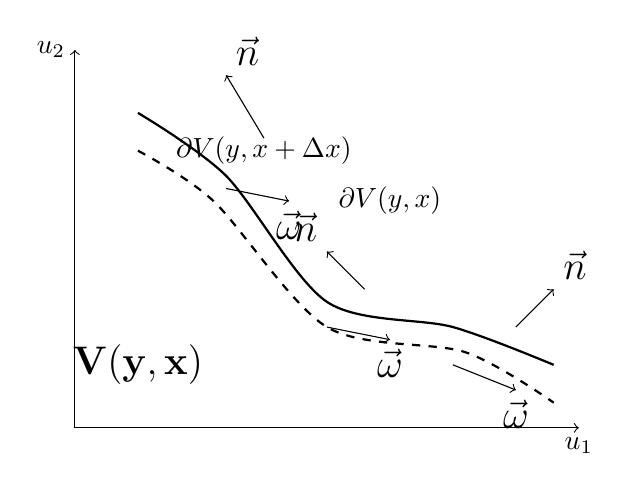
\begin{tikzpicture}[scale=1.6]
 		% Axes
 		\draw[->] (0,0) -- (4,0) node[below] {$u_1$};
 		\draw[->] (0,0) -- (0,3) node[left] {$u_2$};
 		
 		% Labels in the plane
 		\node at (0.5,0.5) {\Large $\mathbf{V(y,x)}$};
 		\node at (1.5,2.2) {$\partial V(y,x+\Delta x)$};
 		\node at (2.5,1.8) {$\partial V(y,x)$};
 		
 		% Curves: solid boundary and dashed boundary
 		\draw[thick] plot [smooth] coordinates {(0.5,2.5) (1.2,2) (2,1) (3,0.8) (3.8,0.5)};
 		\draw[thick, dashed] plot [smooth] coordinates {(0.5,2.2) (1.1,1.8) (2,0.8) (3.1,0.6) (3.8,0.2)};
 		
 		% Arrows for normals n
 		\draw[->] (1.5,2.3) -- (1.2,2.8) node[above right] {\Large $\vec{n}$};
 		\draw[->] (2.3,1.1) -- (2,1.4) node[above left] {\Large $\vec{n}$};
 		\draw[->] (3.5,0.8) -- (3.8,1.1) node[above right] {\Large $\vec{n}$};
 		
 		% Arrows for tangents \omega
 		\draw[->] (1.2,1.9) -- (1.7,1.8) node[below] {\Large $\vec{\omega}$};
 		\draw[->] (2,0.8) -- (2.5,0.7) node[below] {\Large $\vec{\omega}$};
 		\draw[->] (3,0.5) -- (3.5,0.3) node[below] {\Large $\vec{\omega}$};
 	\end{tikzpicture}\hspace{1cm}
 		\caption{ }
 	\end{subfigure}
 	\begin{subfigure}[t]{.44\textwidth}
 		
 		\centering
 		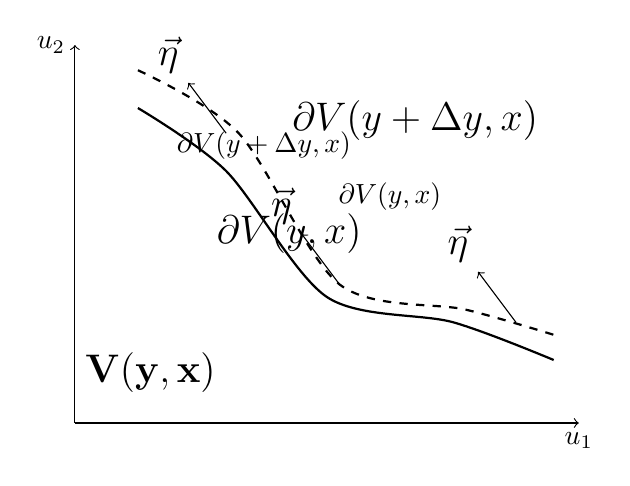
\begin{tikzpicture}[scale=1.6]
 			% Axes
 			\draw[->] (0,0) -- (4,0) node[below] {$u_1$};
 			\draw[->] (0,0) -- (0,3) node[left] {$u_2$};
 			
 			% Labels in the plane
 			\node at (0.6,0.4) {\Large $\mathbf{V(y,x)}$};
 			\node at (1.5,2.2) {$\partial V(y+\Delta y,x)$};
 			\node at (2.5,1.8) {$\partial V(y,x)$};
 			
 			% Curves: solid boundary and dashed boundary
 			\draw[thick] plot [smooth] coordinates {(0.5,2.5) (1.2,2) (2,1) (3,0.8) (3.8,0.5)};
 			\draw[thick, dashed] plot [smooth] coordinates {(0.5,2.8) (1.3,2.3) (2.1,1.1) (3.1,0.9) (3.8,0.7)};
 			
 			% Arrows for normals eta
 			\draw[->] (1.2,2.3) -- (0.9,2.7) node[above left] {\Large $\vec{\eta}$};
 			\draw[->] (2.1,1.1) -- (1.8,1.5) node[above left] {\Large $\vec{\eta}$};
 			\draw[->] (3.5,0.8) -- (3.2,1.2) node[above left] {\Large $\vec{\eta}$};
 			
 			% Labels along boundaries
 			\node at (1.7,1.5) {\Large $\partial V(y,x)$};
 			\node at (2.7,2.4) {\Large $\partial V(y+\Delta y,x)$};
 			
 			
 		\end{tikzpicture}	
 		\caption{ }
 	\end{subfigure}
 	
 	
 	\caption{ \cite{Sasaki2015WhatQuantileRegressions}}
   
 \end{figure}
 
 If $X$ and $U$ are endogenous, then numerator also changes in distribution of $f$. 
  
   
   
    
   	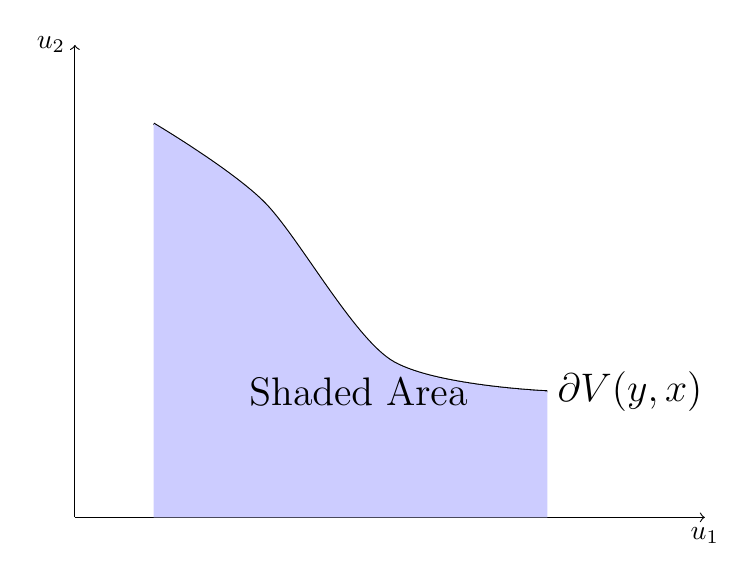
\begin{tikzpicture}[scale=2]
   		% Axes
   		\draw[->] (0,0) -- (4,0) node[below] {$u_1$};
   		\draw[->] (0,0) -- (0,3) node[left] {$u_2$};
   		
   		% Solid curve
   		\draw[thick] plot [smooth] coordinates {(0.5,2.5) (1.2,2) (2,1) (3,0.8)} node[right] {\Large $\partial V(y, x)$};
   		
   		% Shaded area under the curve
   		\fill[blue!20] (0.5,0) -- (0.5,2.5) -- plot [smooth] coordinates {(0.5,2.5) (1.2,2) (2,1) (3,0.8)} -- (3,0.8) -- (3,0) -- cycle;
   		
   		% Label for the shaded area
   		\node at (1.8,0.8) {\Large Shaded Area};
   		
   	\end{tikzpicture}
   	 
    
 
 \subsection{Exploiting Stationary Panel Data}
 
 Like with average effects, the availability of stationary panel data allows one to eliminate the average effect of interest without the heterogeneity bias. 
See \cite{Chernozhukov2015}. 
 
 
 
 \newpage
 
 Maybe \cite{Chernozhukov2018SortedEffectsMethod}?
 
 
 \newpage 
 
 \section{Identification of QTEs under Endogeneity: IV-QR}
 \label{quantile:section:iv_qr}
 
 \subsection{IV}
 
 SWIG here
 
 but see \cite{Wuthrich2020ComparisonTwoQuantile} about what happens the rank similarity does not hold. 
 %
 In this case 
 
 see the Handbook of Quantile Regression \cite{Koenker2017HandbookQuantileRegression}
 
 
 
 see \cite{Pereda-Fernandez2024EstimationCounterfactualDistributions} about endogeneity in distribution regression settings
 
 
 \paragraph{GQR}
 one approach that nests both -- generalized quantile regression \citep{Powell2020}. 
 
 
 
 